\chapter{Examples}
\label{chapter_examples}

The goal in this chapter is to present several examples for the MITHRA users to more easily get familiar with the interface of the software.
%
In addition, through the presented examples the pros and cons of using the developed FDTD/PIC algorithm are more accurately evaluated.
%
For example, the computation time, numerical stability and numerical convergence and more importantly the reliability of results are studied based on some standard examples.
%
The software developers aim to update this chapter with the most recent examples where MITHRA is used for the FEL simulation.
%
The job files needed by the MITHRA code for the examples provided in this chapter are all available in the github repository under the link \href{https://github.com/aryafallahi/mithra}{https://github.com/aryafallahi/mithra}.

\section{Example 1: Infrared FEL}

\subsection{Problem Definition}

\begin{table}
\label{example1}
\caption{Parameters of the Infrared FEL configuration considered as the first example.}
\centering
\begin{tabular}{|c||c|}
\hline
FEL parameter & Value \\ \hline \hline
Current profile & Uniform \\ \hline
Bunch size & (260$\times$260$\times$100.5)\,{\textmu}m \\ \hline
Bunch charge & 29.5\,pC \\ \hline
Bunch energy & 51.4\,MeV \\	\hline
Bunch current & 88.5\,A \\ \hline
Longitudinal momentum spread & 0.01\% \\ \hline
Normalized emittance & 0.0 \\	\hline
Undulator period & 3.0\,cm \\ \hline
Magnetic field & 0.5\,T \\ \hline
Undulator parameter & 1.4 \\ \hline
Undulator length & 5\,m \\ \hline
Radiation wavelength & 3\,$\mu$ m \\ \hline
Electron density & $2.72\times10^{13} 1/\text{cm}^3$ \\ \hline
Gain length (1D) & 22.4\,cm \\ \hline
FEL parameter & 0.006 \\ \hline
Cooperation length & 39.7\,{\textmu}m \\ \hline
Initial bunching factor & $0.01$ \\ \hline
\end{tabular}
\end{table}
%%
As the first example, we consider an infrared FEL with the parameters tabulated in table \ref{example1}, which is inspired by the numerical analysis presented in \cite{tran1989tda}.
%
The bunch distribution is assumed to be uniform in order to compare the results with one-dimensional FEL theory.
%
For the same purpose, the transverse energy spread is considered to be zero and a minimal longitudinal energy spread is assumed.
%
In this first example, saturation of the FEL gain is obtained after a small number of microbunches compared to a typical x-ray FEL, which leads to a short simulation time.
%
As a results, we use this problem to assess the simulation results, verify the convergence and reliability of the algorithm, and finally compare the output with well-established softwares in the community.

To simulate the considered FEL configuration, the following job file is written and given to the software to analyze the interaction and produce the results shown in Fig.\,\ref{power-example1} \footnote{It should be emphasized here that Genesis and MITHRA start the simulation of FEL at different instances. The former considers bunch within the undulator at the start of the simulation, whereas the latter starts the simulation when the bunch is outside the undulator. In the plots presented in this manual, the curves are shifted to have similar gain regimes thereby achieving a valid comparison between the results.}.
%
As observed in the mesh definition, the transverse size of the computational domain is almost 10 times larger than the bunch transverse size.
%
In the contrary, the longitudinal size of the mesh is only three times larger than the bunch length.
%
This needs to be considered due to the failure of absorbing boundary conditions for the oblique incidence of the field.
%
During the simulation, the code adds tapering sections to both bunch and undulator to avoid abrupt transitions which produce coherent scattering emission (CSE).
%
To consider such the additional tepreing sections, the undulator begin is initialized at least ten radiation wavelengths apart from the bunch head to reduce the CSE.
%
This also introduces corresponding limitations on the mesh size, meaning that the minimum distance from the bunch tail and the mesh boundary should be at least ten radiation wavelengths.
%
In the illustrated job file, some of the output formats are turned off which can always be activated to obtain the required data.
%
\begin{snugshade}
\begin{Verbatim}[fontsize=\small, tabsize=4, fontfamily=courier, fontseries=b, commandchars=\\\{\}, obeytabs]
MESH
\{
	length-scale					= MICROMETER
	time-scale						= PICOSECOND
	mesh-lengths					= ( 3200,  3200.0,    280.0)
	mesh-resolution					= ( 50.0,    50.0,      0.1)
	mesh-center						= ( 0.0,      0.0,      0.0)
	total-time						= 30000
	bunch-time-step					= 1.6
	bunch-time-start				= 0.0
	mesh-truncation-order			= 2
	space-charge					= false
	solver							= NSFD
\}

BUNCH
\{
	bunch-initialization
	\{
		type						= ellipsoid
		distribution				= uniform
		charge						= 1.846e8
		number-of-particles			= 131072
		gamma						= 100.41
		direction					= (    0.0,     0.0,       1.0)
		position					= (    0.0,     0.0,       0.0)
		sigma-position				= (  260.0,   260.0,     50.25)
		sigma-momentum				= ( 1.0e-8,  1.0e-8, 100.41e-4)
		transverse-truncation		= 1040.0
		longitudinal-truncation		= 90.0
		bunching-factor				= 0.01
	\}
\}

FIELD
\{
	field-sampling
	\{
		sample						= true
		type						= at-point
		field						= Ex
		field						= Ey
		field						= Ez
		directory					= ./
		base-name					= field-sampling/field
		rhythm						= 3.2
		position					= (0.0, 0.0, 110.0)
	\}
\}

UNDULATOR
\{
	undulator-parameter				= 1.417
	period							= 3.0e4
	length							= 300
	polarization-angle				= 0.0
\}

FEL-OUTPUT
\{
	radiation-power
	\{
		sample						= true
		type						= at-point
		directory					= ./
		base-name					= power-sampling/power
		distance-from-bunch			= 110.0
		normalized-frequency		= 1.00
	\}
\}
\end{Verbatim}
\end{snugshade}

\subsection{Simulation Results}

In the beginning, we neglect the space-charge effect only to achieve a good assessment of MITHRA simulation results.
%
The investigation of space-charge effect will be performed in the second step.
%
Fig.\,\ref{power-example1}a shows the transverse electric field sampled at 110\,{\textmu}m in front of the bunch center.
%
The logarithmic plot of the radiated power for different propagation lengths ($z$) is also depicted in Fig.\,\ref{power-example1}b.
%
We comment that the full-wave analysis offered by MITHRA obtains the total radiated field as a superposition of forward, backward and near-field radiation components.
%
In an FEL simulation, one is often interested in the forward radiation component, which can only be extracted at a distance in front of the radiation source, namely the electron bunch.
%
This is the main reason for illustrating the radiated power and field at 110\,{\textmu}m in front of the bunch center.

According to the 1D FEL theory the gain length of the considered SASE FEL configuration is $L_G=22.4\,\mathrm{cm}$.
%
The gain length calculated from the slope of the power curve is $L_G=22\,\mathrm{cm}$.
%
There exists also a good agreement in the computed saturation power.
%
The beam energy according to the data in table \ref{example1} is 1.52\,mJ which for the bunch length of 100\,{\textmu}m corresponds to $P_{beam}=4.55\,\mathrm{GW}$ beam power.
%
The estimated saturation power according to the 1D theory is equal to $P_{sat} = \rho P_{beam} = 2.7\,\mathrm{GW}$.
%
The saturation power computed by MITHRA is $2.6\,\mathrm{GW}$.

We have also performed a comparison study between the obtained results from MITHRA and the code Genesis 1.3, which is presented in Fig.\,\ref{power-example1}b.
%
As observed, both codes produce similar results in the initial state and the gain regime.
%
Nonetheless, there exists a considerable discrepancy between the calculated radiated power in the saturation regime.
%
The illustrated results in Fig.\,\ref{power-example1}b show that the steady state and time domain analyses using Genesis do not produce similar results.
%
This shows that the bunch is not long enough to justify the steady state approximation, and dictates a time domain analysis for accurate simulation.
%
However, the results obtained by MITHRA at saturation do not match with the Genesis results even in the time domain.

The origin of such a discrepancy is described as follows:
%
As explained in chapter \ref{chapter_introduction}, Genesis 1.3 and all the existing softwares for FEL simulation neglect the backward radiation of the electrons.
%
Such an approximation is motivated by the inherent interest in forward radiation in the FEL process.
%
However, the backward radiation although is seldom used due to its long wavelength, it influences the motion of electrons, the charge distribution and in turn the FEL output.
%
The influence of low-frequency backward radiation on the performance of free electron lasers has been already studied in a 1D regime \cite{maroli2000effects}.
%
The effect becomes stronger in the saturation regime, where the electron bunch is modulated and the FEL radiation is a strong function of the particles distribution.
%
To demonstrate this effect, we used a mathematical trick in MITHRA through the domain decomposition algorithm to suppress the propagation of backward radiation.
%
The results of such an analysis is also shown in Fig.\,\ref{power-example1}b, which shows a relatively better agreement with time domain simulation results returned by Genesis 1.3.
%
The still existing discrepancy is attributed to the different formulations of FDTD and TDA algorithms as well as the introduced tapers in bunch current and undulator fields.
%
\begin{figure}
\centering
$\begin{array}{cc}
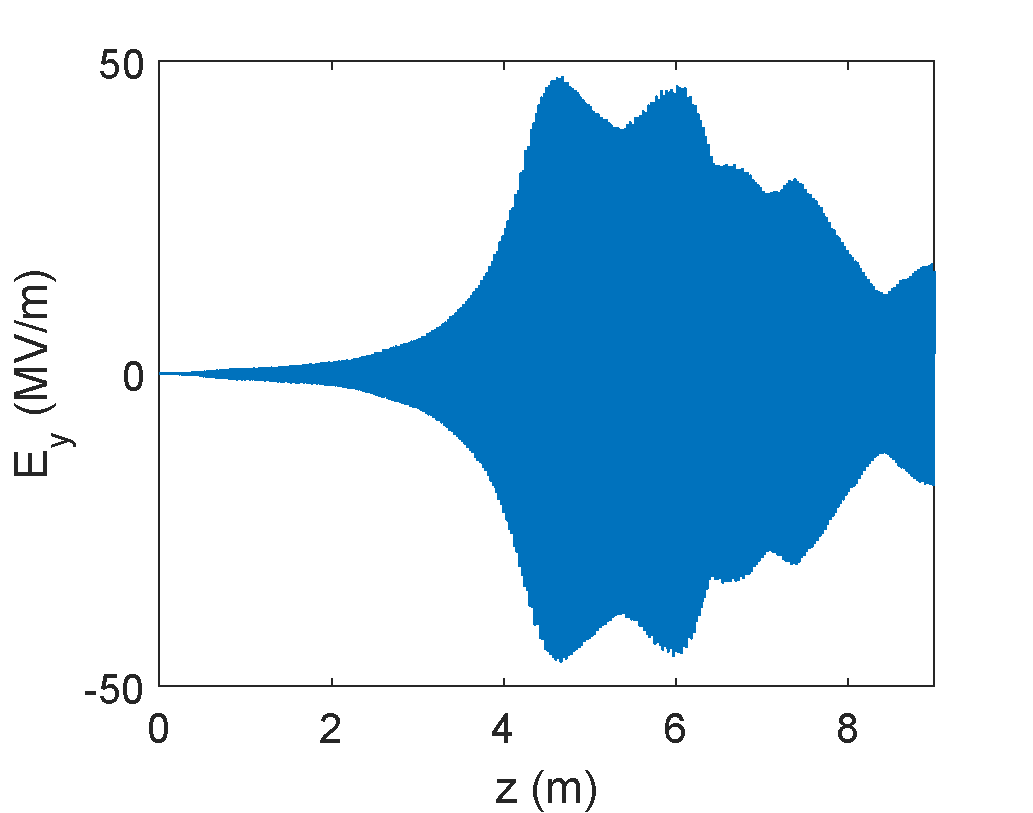
\includegraphics[height=2.5in]{./MITHRA_EXAMPLES/Fig1/Fig1a.pdf} & 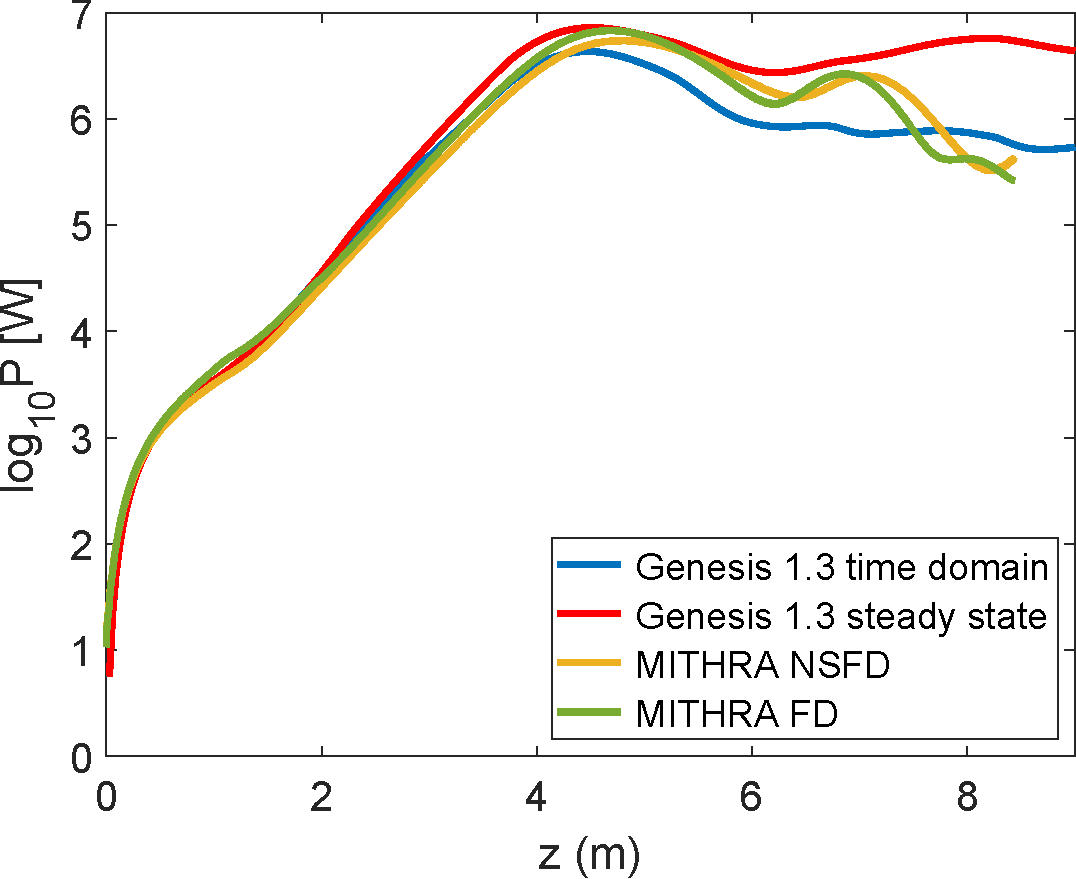
\includegraphics[height=2.5in]{./MITHRA_EXAMPLES/Fig1/Fig1b.pdf} \\
(a) & (b)
\end{array}$
\caption{(a) The transverse field $E_y$ at 110\,$\mu$m distance from the bunch center and (b) the total radiated power calculated at 110\,$\mu$m distance from the bunch center in terms of the traveled undulator length.}
\label{power-example1}
\end{figure}

There exists a discrepancy between MITHRA and Genesis 1.3 results at the beginning of the undulator.
%
The reason for this discrepancy in the initial radiation is that MITHRA initializes the bunch outside the undulator.
%
After passing through the fringing fields of the undulator, CSE happens which causes MITHRA to show the beginning of radiation from a value different from zero, whereas in Genesis 1.3 and in many of the typical FEL codes radiation starts from zero.
%
We preferred such an operation basis in MITHRA to consider for the CSE effect in real FEL simulations.
%
Furthermore, in Fig.\,\ref{power-example1}b, we compare the results obtained using the NSFD implemented in MITHRA and standard FD scheme.
%
As observed, formulation based on FD predicts higher radiation power compared to NSFD.
%
This effect happens due to the smaller phase velocity of light when wave propagation follows dispersion equation (\ref{numericalDispersionCD}).
%
The result is slower phase slippage of electron bunch over the radiation and consequently later saturation of the radiation.

As a 3D electromagnetic simulation, it is always beneficial to investigate the electromagnetic field profile in the computational domain.
%
Using the field visualization capability in MITHRA, snapshots of the field profile at different instants and from various view points are provided.
%
In Fig.\,\ref{profile-example1}, snapshots of the radiated field profile, beam power and bunch profile at different time instants are illustrated.
%
The emergence of lasing radiation at the end of the undulator motion is clearly observed in the field profile.
%
\begin{figure}
\centering
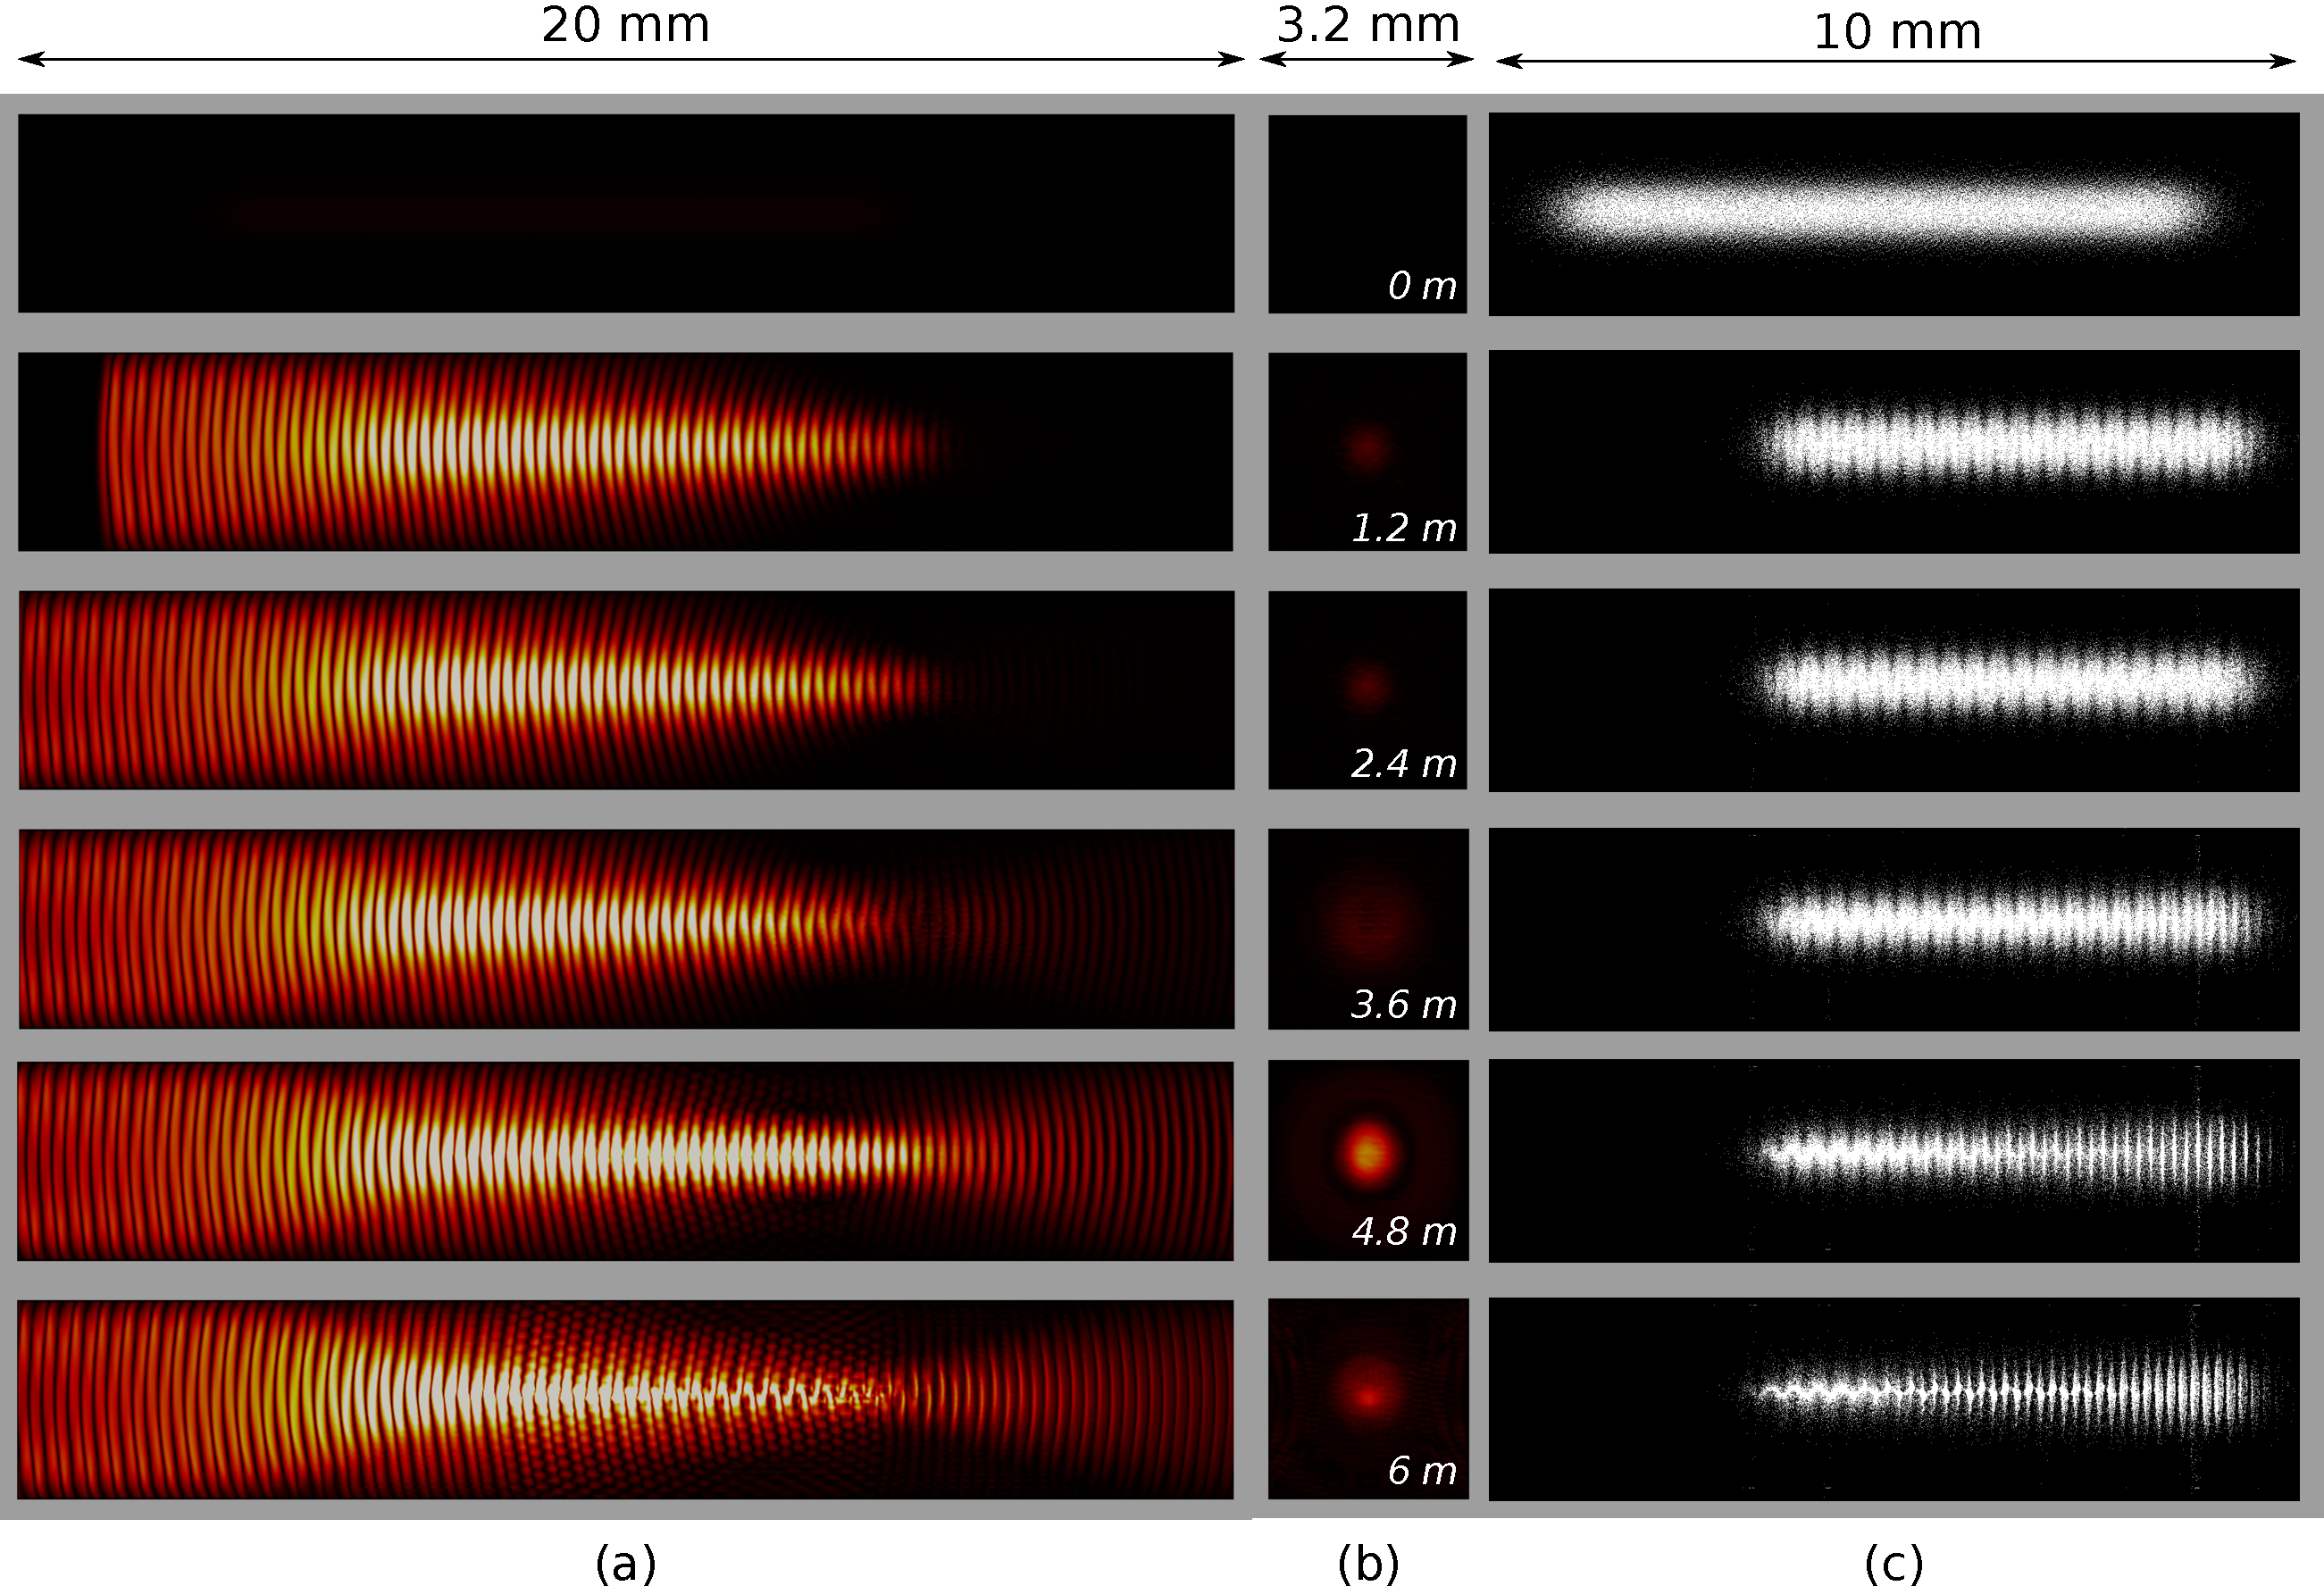
\includegraphics[width=7.0in]{./MITHRA_EXAMPLES/Fig2/Fig2.pdf}
\caption{(a) Snapshots of the radiated field profile taken at $x=0$ , (b) snapshots of the beam power at $z=60\,\mu m$ plane, and (c) the bunch profile viewed from the $x$ axis.}
\label{profile-example1}
\end{figure}
%
Furthermore, snapshots of the bunch profile are also presented beside the field profile.
%
The main FEL principle which is the lasing due to micro-bunching of the electron bunch is observed from the field and bunch profiles.
%
The first two snapshots evidence a considerable change in the bunch length, which occurs due to the entrance in the undulator.
%
The bunch outside of the undulator with Lorentz factor $\gamma$ travels faster than the bunch inside the undulator with Lorentz factor $\gamma/\sqrt{1+K^2/2}$.
%
Therefore, after the entrance to the undulator the bunch length becomes shorter.
%
This effect may not be easily observed in real laboratory frame, but is significant in electron rest frame.

\subsection{Convergence Analysis}

The convergence rate of the results is the main factor used to assess a numerical algorithm. %%
%%
In our FEL analysis, there are several parameters introduced by the numerical method which may affect the final result. %%
%%
These parameters include (1) number of macro-particles ($n$), (2) time step for updating equation of motion ($\Delta t_b$), (3) longitudinal mesh size ($l_z$), (4) transverse mesh size ($l_x=l_y$), (5) longitudinal discretization ($\Delta z$) and (6) transverse discretization ($\Delta x = \Delta y$). %%
%%
Studying the convergence of the results is crucial to acquire an estimate for the uncertainty in the reported values. %%
%%
Here, this task is accomplished by sweeping over the above parameters and plotting the error function defined as the following:
%%
\begin{equation}
\label{errorDefinition}
\mathrm{error} = \frac{\int_{z_i}^{z_f} | P(z)-P_0(z) | \mathrm{dz}}{\int_{z_i}^{z_f} P_0(z) \mathrm{dz}},
\end{equation}
%%
where $z_i$ and $z_f$ are the beginning and end of the undulator, respectively and $P_0$ is the reference simulation result which is chosen as the results with the highest resolution. %%

In Fig.\,\ref{convergenceStudy} the convergence study is shown for the aforementioned parameters. %%
\begin{figure}
\centering
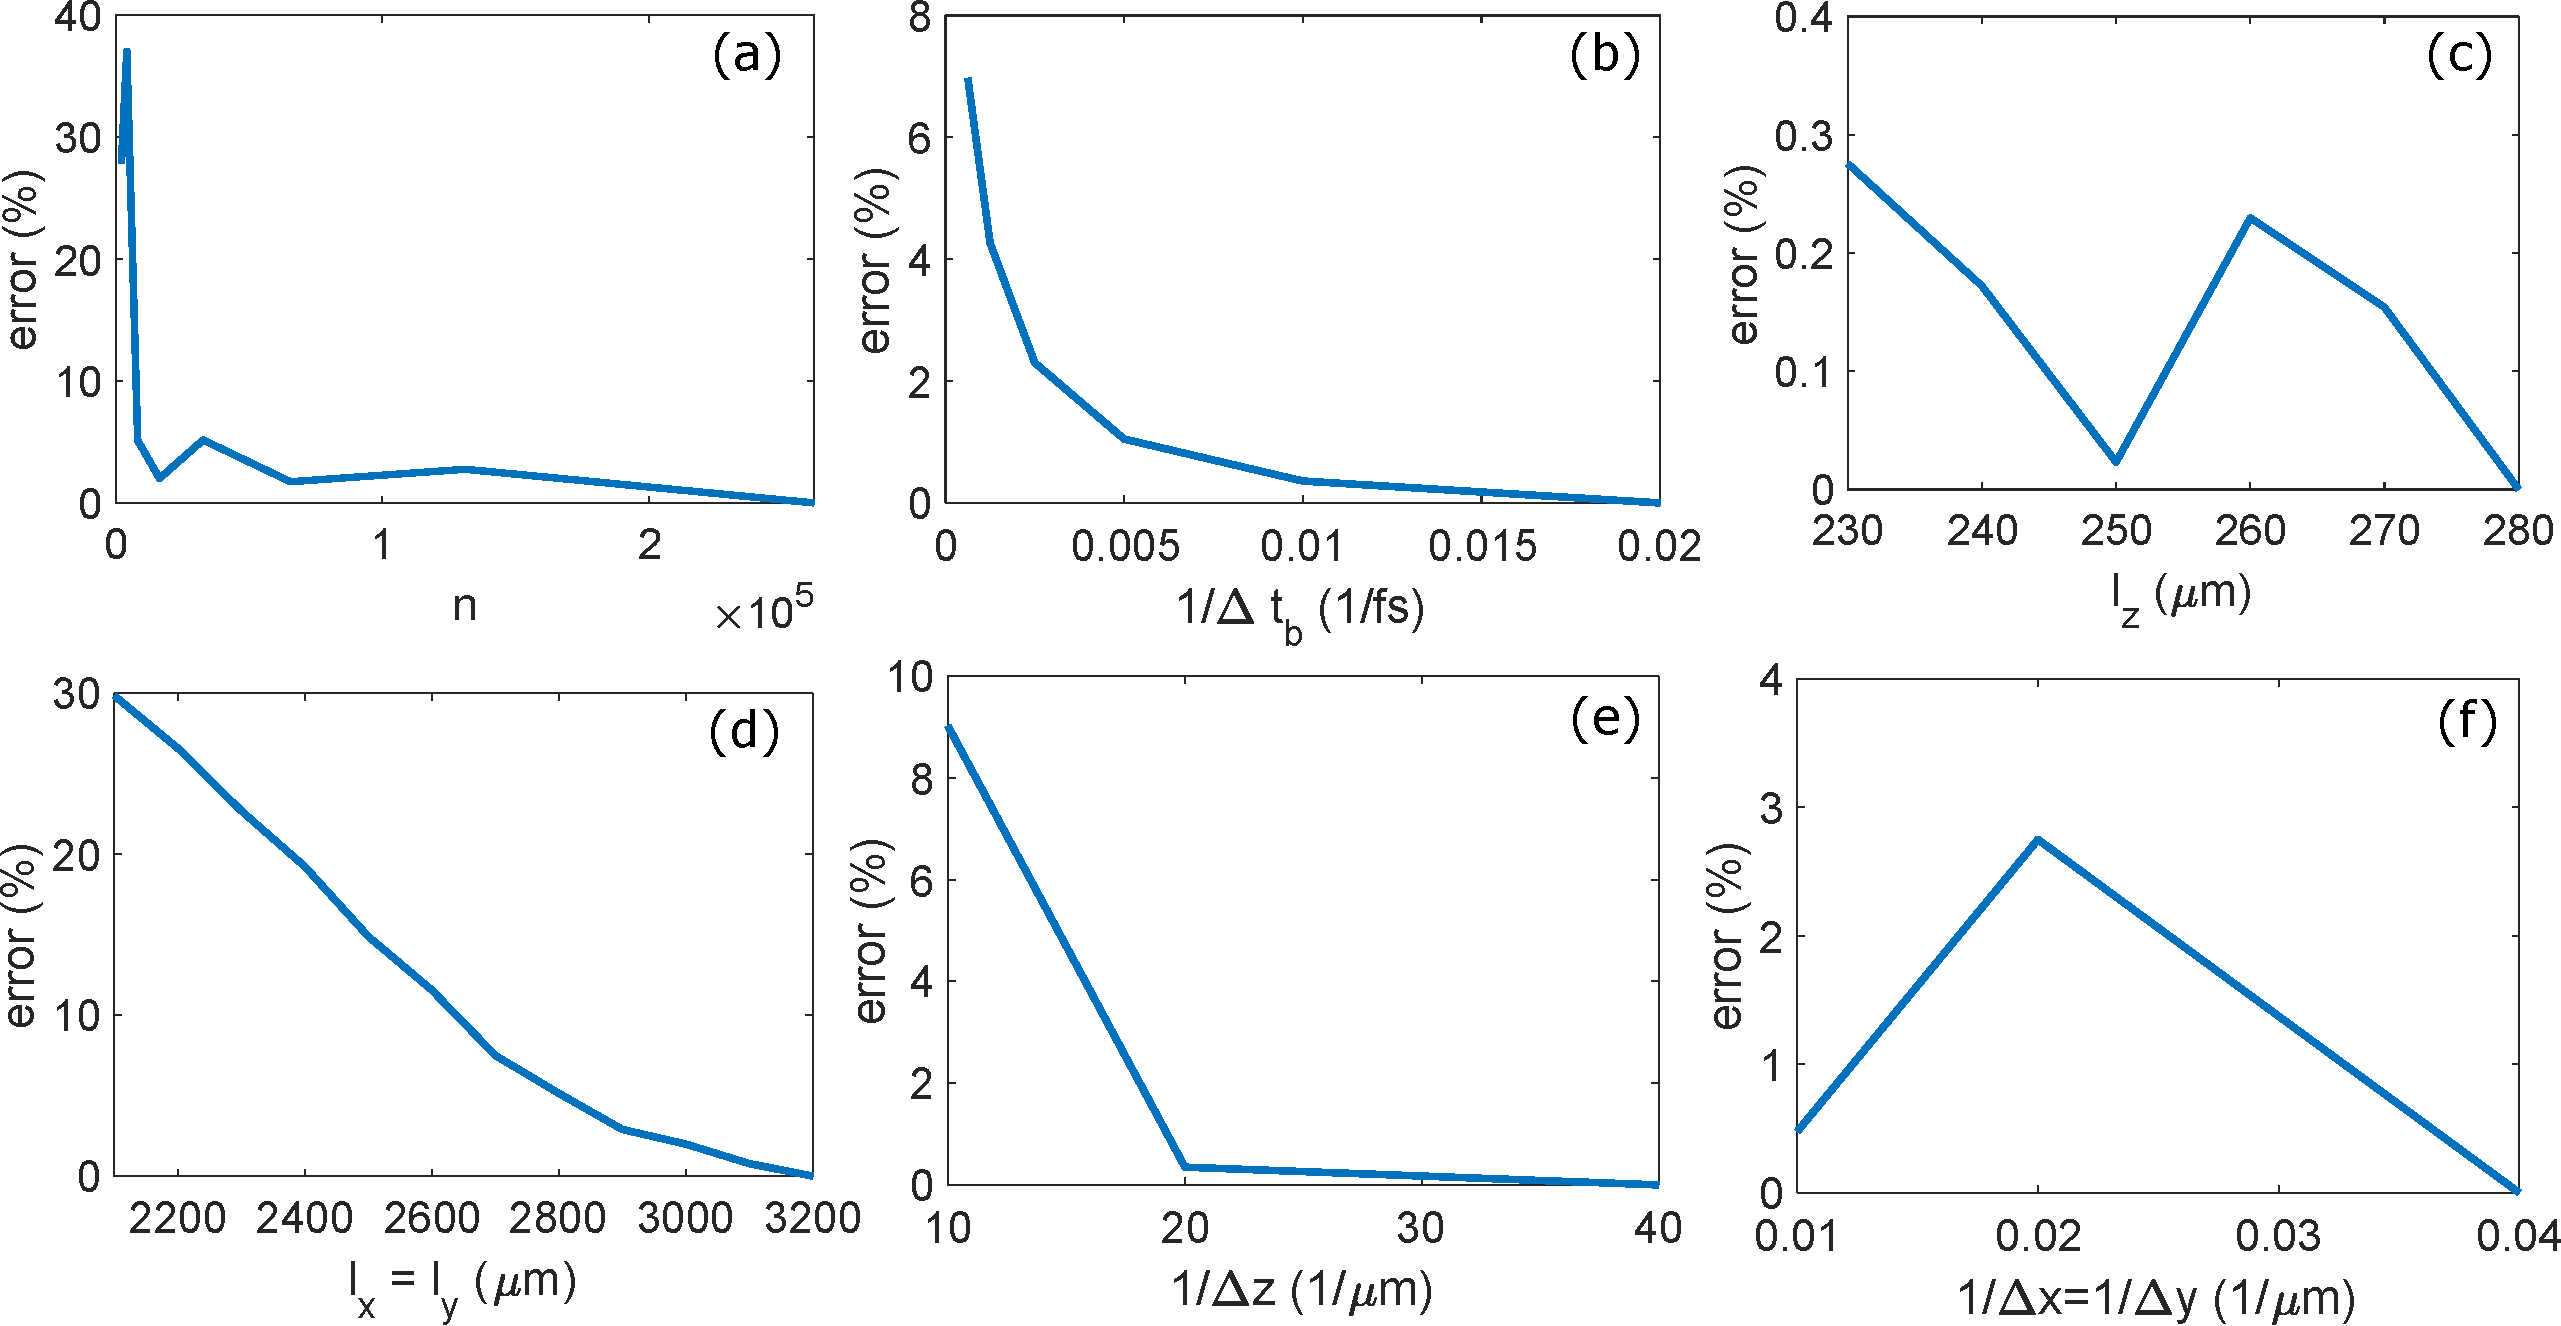
\includegraphics[width=7.0in]{./MITHRA_EXAMPLES/Fig3/Fig3.pdf}
\caption{Convergence study for the different involved parameters in the considered FEL simulation: (a) $n$, (b) $\Delta t_b$, (c) $l_z$, (d) $l_x=l_y$, (e) $\Delta z$ and (f) $\Delta x = \Delta y$}
\label{convergenceStudy}
\end{figure}
%
Generally, accuracy of less than 3\% is achieved by using the initially suggested values.

\subsection{Space-charge effect}

A promising benefit offered by MITHRA is the assessment of various approximations used in the previously developed FEL codes.
%
As an example, the algorithm used in the TDA method to evaluate the space-charge effect can be examined and verified using this code.
%
The TDA method implemented in Genesis 1.3 software considers a periodic variation of space-charge force throughout the electron bunch \cite{tranFEL,reiche2000numerical}.
%
This assumption is implicitly made, when electric potential equation is solved in a discrete Fourier space.
%
However, a simple investigation of bunch profiles shown in Fig.\,\ref{profile-example1}c shows that a periodic assumption for the electron distribution may be a crude approximation.
%
In addition, this assumption is favored by the FEL gain process and potentially decreases any detrimental influence of the space-charge fields on the FEL radiation.
%
On the other hand, the algorithm in TDA method considers longitudinal space-charge forces and neglects transverse forces, which is merely valid in high energy electron regimes.

In Fig.\,\ref{spaceChargeEffect}a, we are comparing the solution of the FEL problem using MITHRA and Genesis 1.3 with and without considering the space-charge effect.
%
As observed in the results, the effect of space-charge on the radiation gain predicted by MITHRA is much stronger than the same effect predicted by Genesis.
%
This is attributed to the assumption of periodic variations in the space-charge force made in TDA algorithm.
%
If such a hypothesis is correct, the observed discrepancy should reduce once the radiation from a longer bunch is simulated, because the accuracy of periodicity assumption increases for longer bunches.
%
Indeed, this is observed after repeating the simulation for longer electron bunches with similar charge and current densities.
%
The results of such a study is illustrated in Fig.\,\ref{spaceChargeEffect}b.
%
Note that in the performed simulations covering the space-charge effects, the grid size along $z$ direction had to be decreased to 50\,{\textmu}m to obtain results with acceptable accuracy.
%
\begin{figure}
\centering
$\begin{array}{cc}
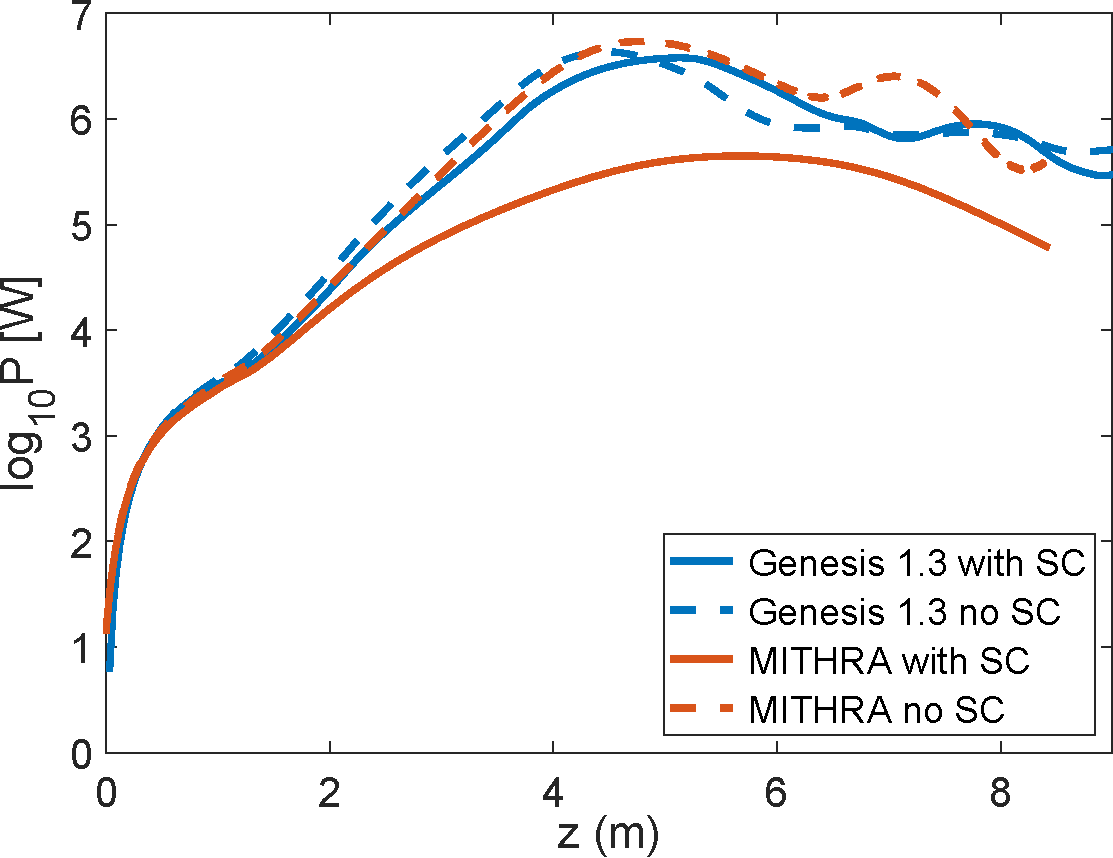
\includegraphics[height=2.5in]{./MITHRA_EXAMPLES/Fig4/Fig4a.pdf} & 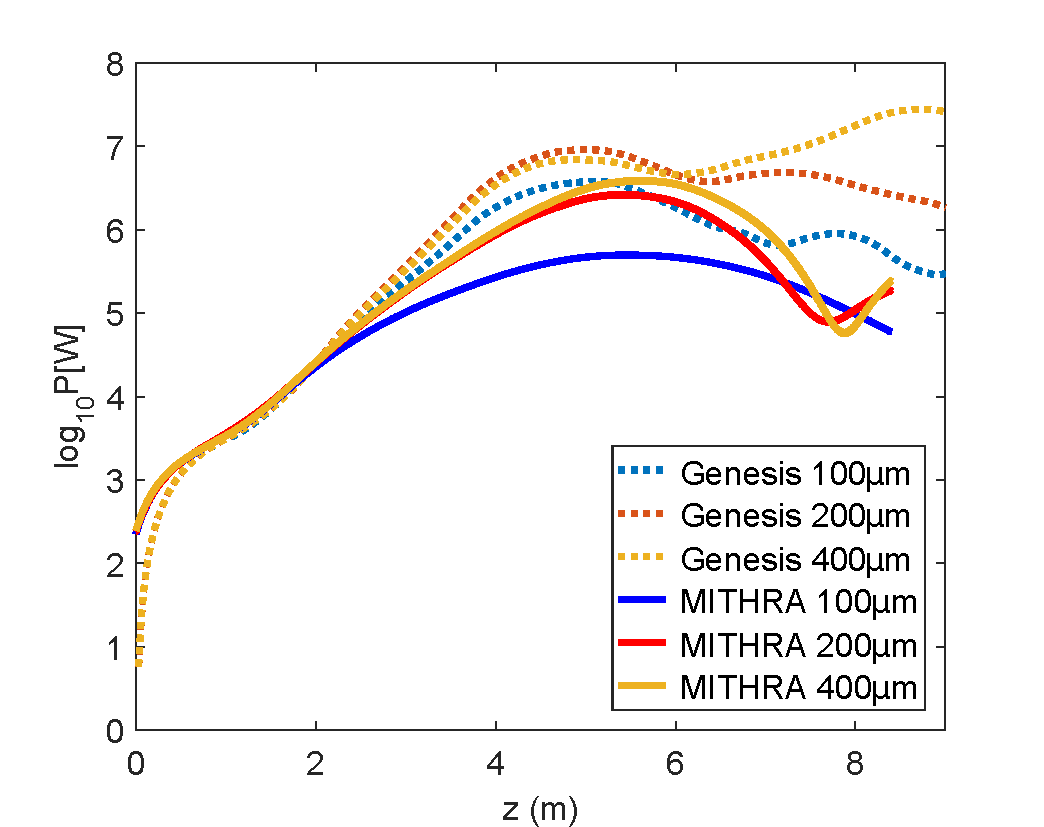
\includegraphics[height=2.5in]{./MITHRA_EXAMPLES/Fig4/Fig4b.pdf} \\
(a) & (b)
\end{array}$
\caption{The total radiated power calculated at 110\,$\mu$m distance from the bunch center in terms of the traveled undulator length (a) with and without space-charge consideration and (b) various lengths of the bunch with space-charge assumption.}
\label{spaceChargeEffect}
\end{figure}

\subsection{Computation performance}

A potential user of the code is usually interested in the total computation resources required for a specific FEL simulation.
%
To clarify such features, the study on the computation performance for MPI parallelized code is presented in Fig.\,\ref{computationPerformance}, where the total computation time is depicted in terms of the number of processors.
%
The simulation with 131072 macro-particles, a grid with 11'468'800 cells and 37'500 time steps is taken into account.
%
The code is run on euler cluster of the scientific computing facility at ETH Z\"urich.
%
It is observed that running on 48 CPUs is optimal for this problem.
%
This number increases for larger and more demanding examples.
%
In case of the run on 40 CPUs, field update on the computational grid, motion update of the bunch macro-particles and the computation of the total radiated field together with the required Fourier transform take 44\%, 28\%, and 28\% of the total computational time, respectively.
%
\begin{figure}
	\centering
	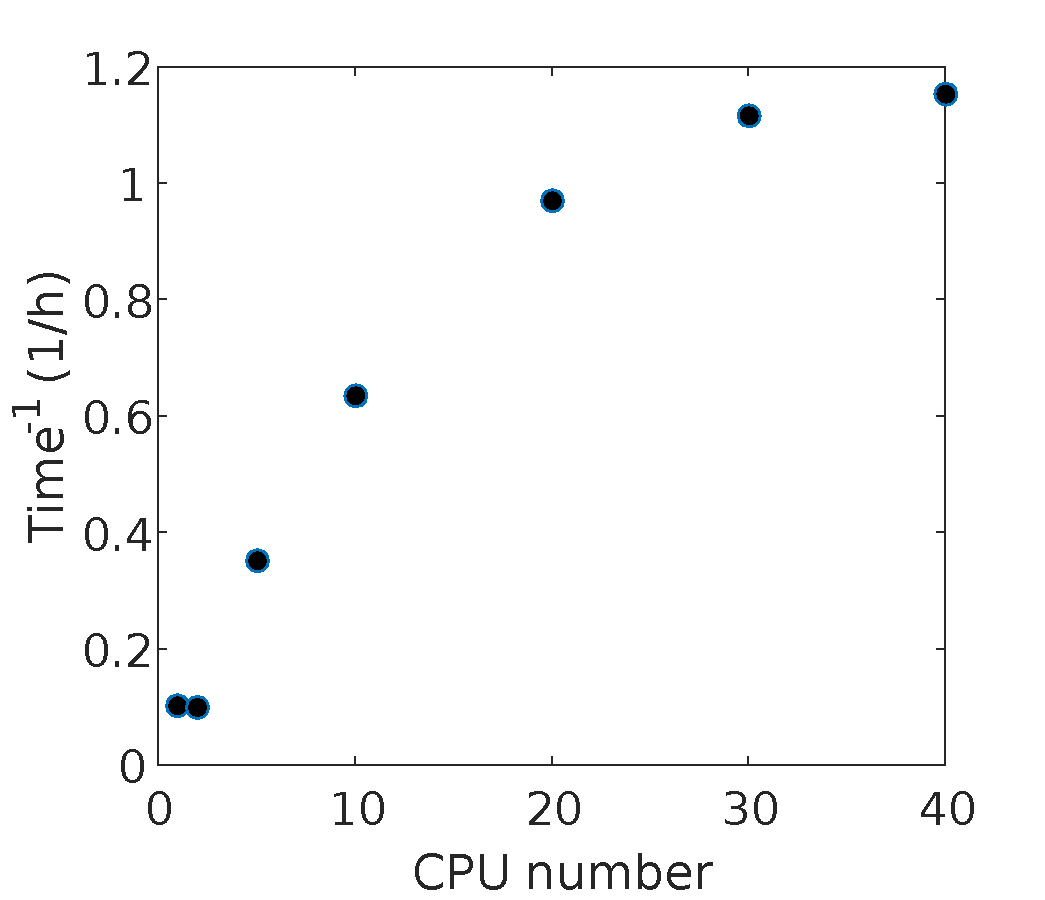
\includegraphics[width=3.0in]{./MITHRA_EXAMPLES/Fig5/Fig5.pdf}
	\caption{Reverse of total computation time versus the total number of processors.}
	\label{computationPerformance}
\end{figure}

\section{Example 2: Seeded UV FEL}

\subsection{Problem Definition}

\begin{table}
\label{example2}
\caption{Parameters of the UV seeded FEL configuration considered as the second example.}
\centering
\begin{tabular}{|c||c|}
\hline
FEL parameter & Value \\ \hline \hline
Current profile & Uniform \\ \hline
Bunch size & (95.3$\times$95.3$\times$150)\,{\textmu}m \\ \hline
Bunch charge & 54.9\,pC \\ \hline
Bunch energy & 200\,MeV \\	\hline
Bunch current & 110\,A \\ \hline
Longitudinal momentum spread & 0.01\% \\ \hline
Normalized emittance & 0.97 {\textmu}m-rad \\	\hline
Undulator period & 2.8\,cm \\ \hline
Magnetic field & 0.7\,T \\ \hline
Undulator parameter & 1.95 \\ \hline
Undulator length & 15\,m \\ \hline
Radiation wavelength & 0.265\,{\textmu}m \\ \hline
Electron density & $2.52\times10^{14} 1/\text{cm}^3$ \\ \hline
Gain length (1D) & 38.6\,cm \\ \hline
FEL parameter & 0.0033 \\ \hline
Cooperation length & 3.65\,{\textmu}m \\ \hline
Initial bunching factor & $0.0$ \\ \hline
Seed type & Gaussian beam \\ \hline
Seed focal point & 70\,cm \\ \hline
Seed beam radius & 183.74\,{\textmu}m \\ \hline
Seed pulse length & infinite \\ \hline
Seed power & 10\,kW \\ \hline
\end{tabular}
\end{table}
%
As the second example, we consider a seeded FEL in the UV regime to verify the implemented features for simulating a seeded FEL.
%
The parameters of the considered case are taken from \cite{andriyash2015spectral}, which are tabulated in table \ref{example2}.
%
The bunch distribution is again assumed to be uniform with a long current profile ($\sim$1000 times the radiation wavelength) in order to compare the results with the steady state simulations.
%
For the same reason, the seed pulse length is considered to be infinitely long, i.e. a continuous wave pulse.
%
The transverse energy spread is calculated for a bunch with normalized transverse emittance equal to 1\,mm\,mrad.
%
Because of the very long bunch compared to the previous example, the number of required micro-particles to obtain convergent results is 8 times larger.
%
Furthermore, the stronger undulator parameter dictates a smaller time step for the simulation of bunch dynamics.
%
Note that MITHRA, takes the bunch step value as an initial guess, it automatically adjusts the value based on the calculated time step for mesh update.
%
To simulate the considered FEL configuration, the following job file is written and given to the software to analyze the interaction.
%
\begin{snugshade}
\begin{Verbatim}[fontsize=\small, tabsize = 4]
MESH
{
  length-scale                     = MICROMETER
  time-scale                       = PICOSECOND
  mesh-lengths                     = ( 1600.0, 1600.0, 165.0)
  mesh-resolution                  = ( 10.0,   10.0,   0.01 )
  mesh-center                      = ( 0.0,    0.0,    0.0  )
  total-time                       = 50000
  bunch-time-step                  = 0.8
  bunch-time-start                 = 0.0
  mesh-truncation-order            = 2
  space-charge                     = true
}

BUNCH
{
  bunch-initialization
  {
    type                           = ellipsoid
    distribution                   = uniform
    charge                         = 3.4332e8
    number-of-particles            = 1048576
    gamma                          = 391.36
    direction                      = ( 0.0,  0.0,  1.0 )
    position                       = ( 0.0,  0.0,  0.0 )
    sigma-position                 = ( 95.3, 95.3, 75.0)
    sigma-momentum                 = ( 0.0105, 0.0105, 391.36e-4)
    transverse-truncation          = 400.0
    longitudinal-truncation        = 78.0
    bunching-factor                = 0.0
  }

  bunch-profile
  {
    sample                         = true
    directory                      = ./
    base-name                      = bunch-profile/bunch
    time                           = 40000
  }
}

FIELD
{
  field-initialization
  {
    type                           = gaussian-beam
    position                       = ( 0.0, 0.0, 700080)
    direction                      = ( 0.0, 0.0, 1.0)
    polarization                   = ( 0.0, 1.0, 0.0)
    rayleigh-radius-parallel       = 183.74
    rayleigh-radius-perpendicular  = 183.74
    strength-parameter             = 9.857e-7
    signal-type                    = gaussian
    offset                         = 700005.0
    variance                       = 1e12
    wavelength                     = 0.265187
    CEP                            = 0.0
  }
}

UNDULATOR
{
  undulator-parameter              = 1.95
  period                           = 2.8e4
  length                           = 535
  polarization-angle               = 0.0
}

FEL-OUTPUT
{
  radiation-power
  {
    sample                         = true
    type                           = at-point
    directory                      = ./
    base-name                      = power-sampling/power
    distance-from-bunch            = 80.0
    normalized-frequency           = 1.00
  }
}
\end{Verbatim}
\end{snugshade}

\subsection{Simulation Results}

Fig.\,\ref{power-example2}a shows the radiated power in terms of travelled undulator distance computed using MITHRA and Genesis.
%
As observed again in this example, the results agree very well in the seeded and gain regime, with notable discrepancies in the saturation regime.
%
In Fig.\,\ref{power-example2}b, the bunch profile after 12\,m propagation in the undulator is also depicted.
%
The micro-bunching of the large bunch is only visible once a zoom into a part of the bunch is considered.
%
The investigation of the results with and without considering space-charge effect shows that in the seeded and gain intervals, space charge plays a negligible role.
%
However, in the saturation regime the effect of space-charge predicted by MITHRA is stronger than the effect predicted by Genesis.
%
\begin{figure}
\centering
$\begin{array}{cc}
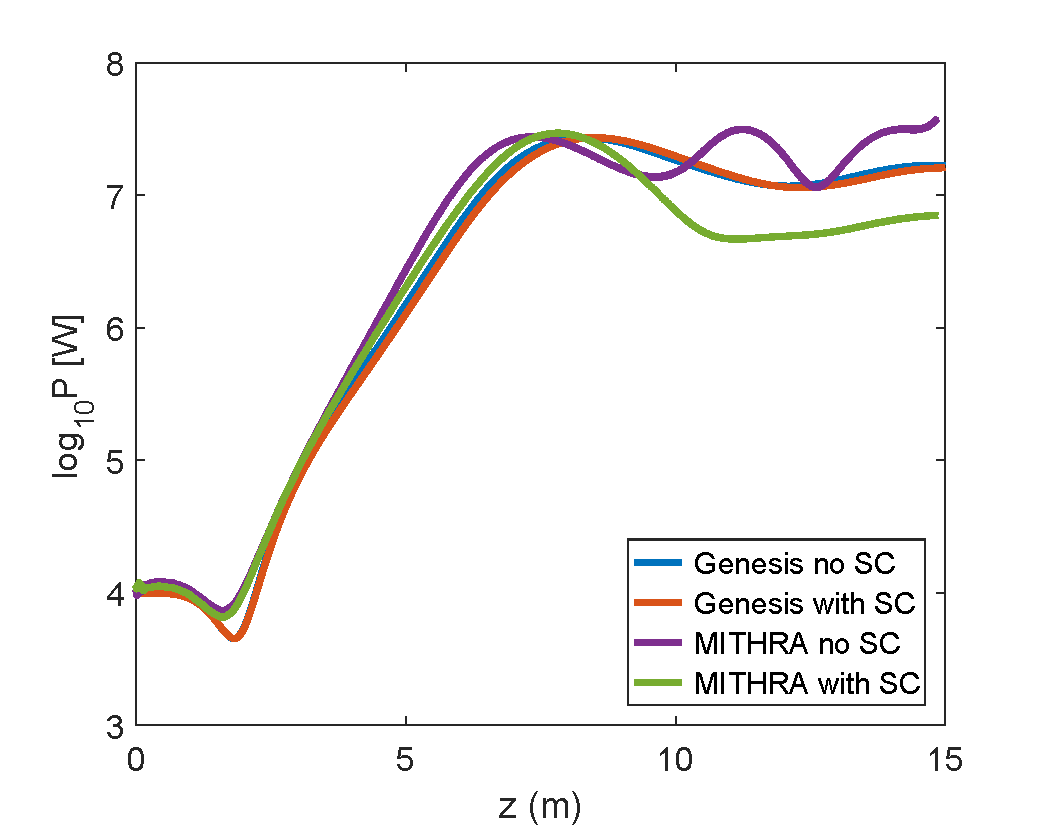
\includegraphics[height=2.5in]{./MITHRA_EXAMPLES/Fig6/Fig6a.pdf} & 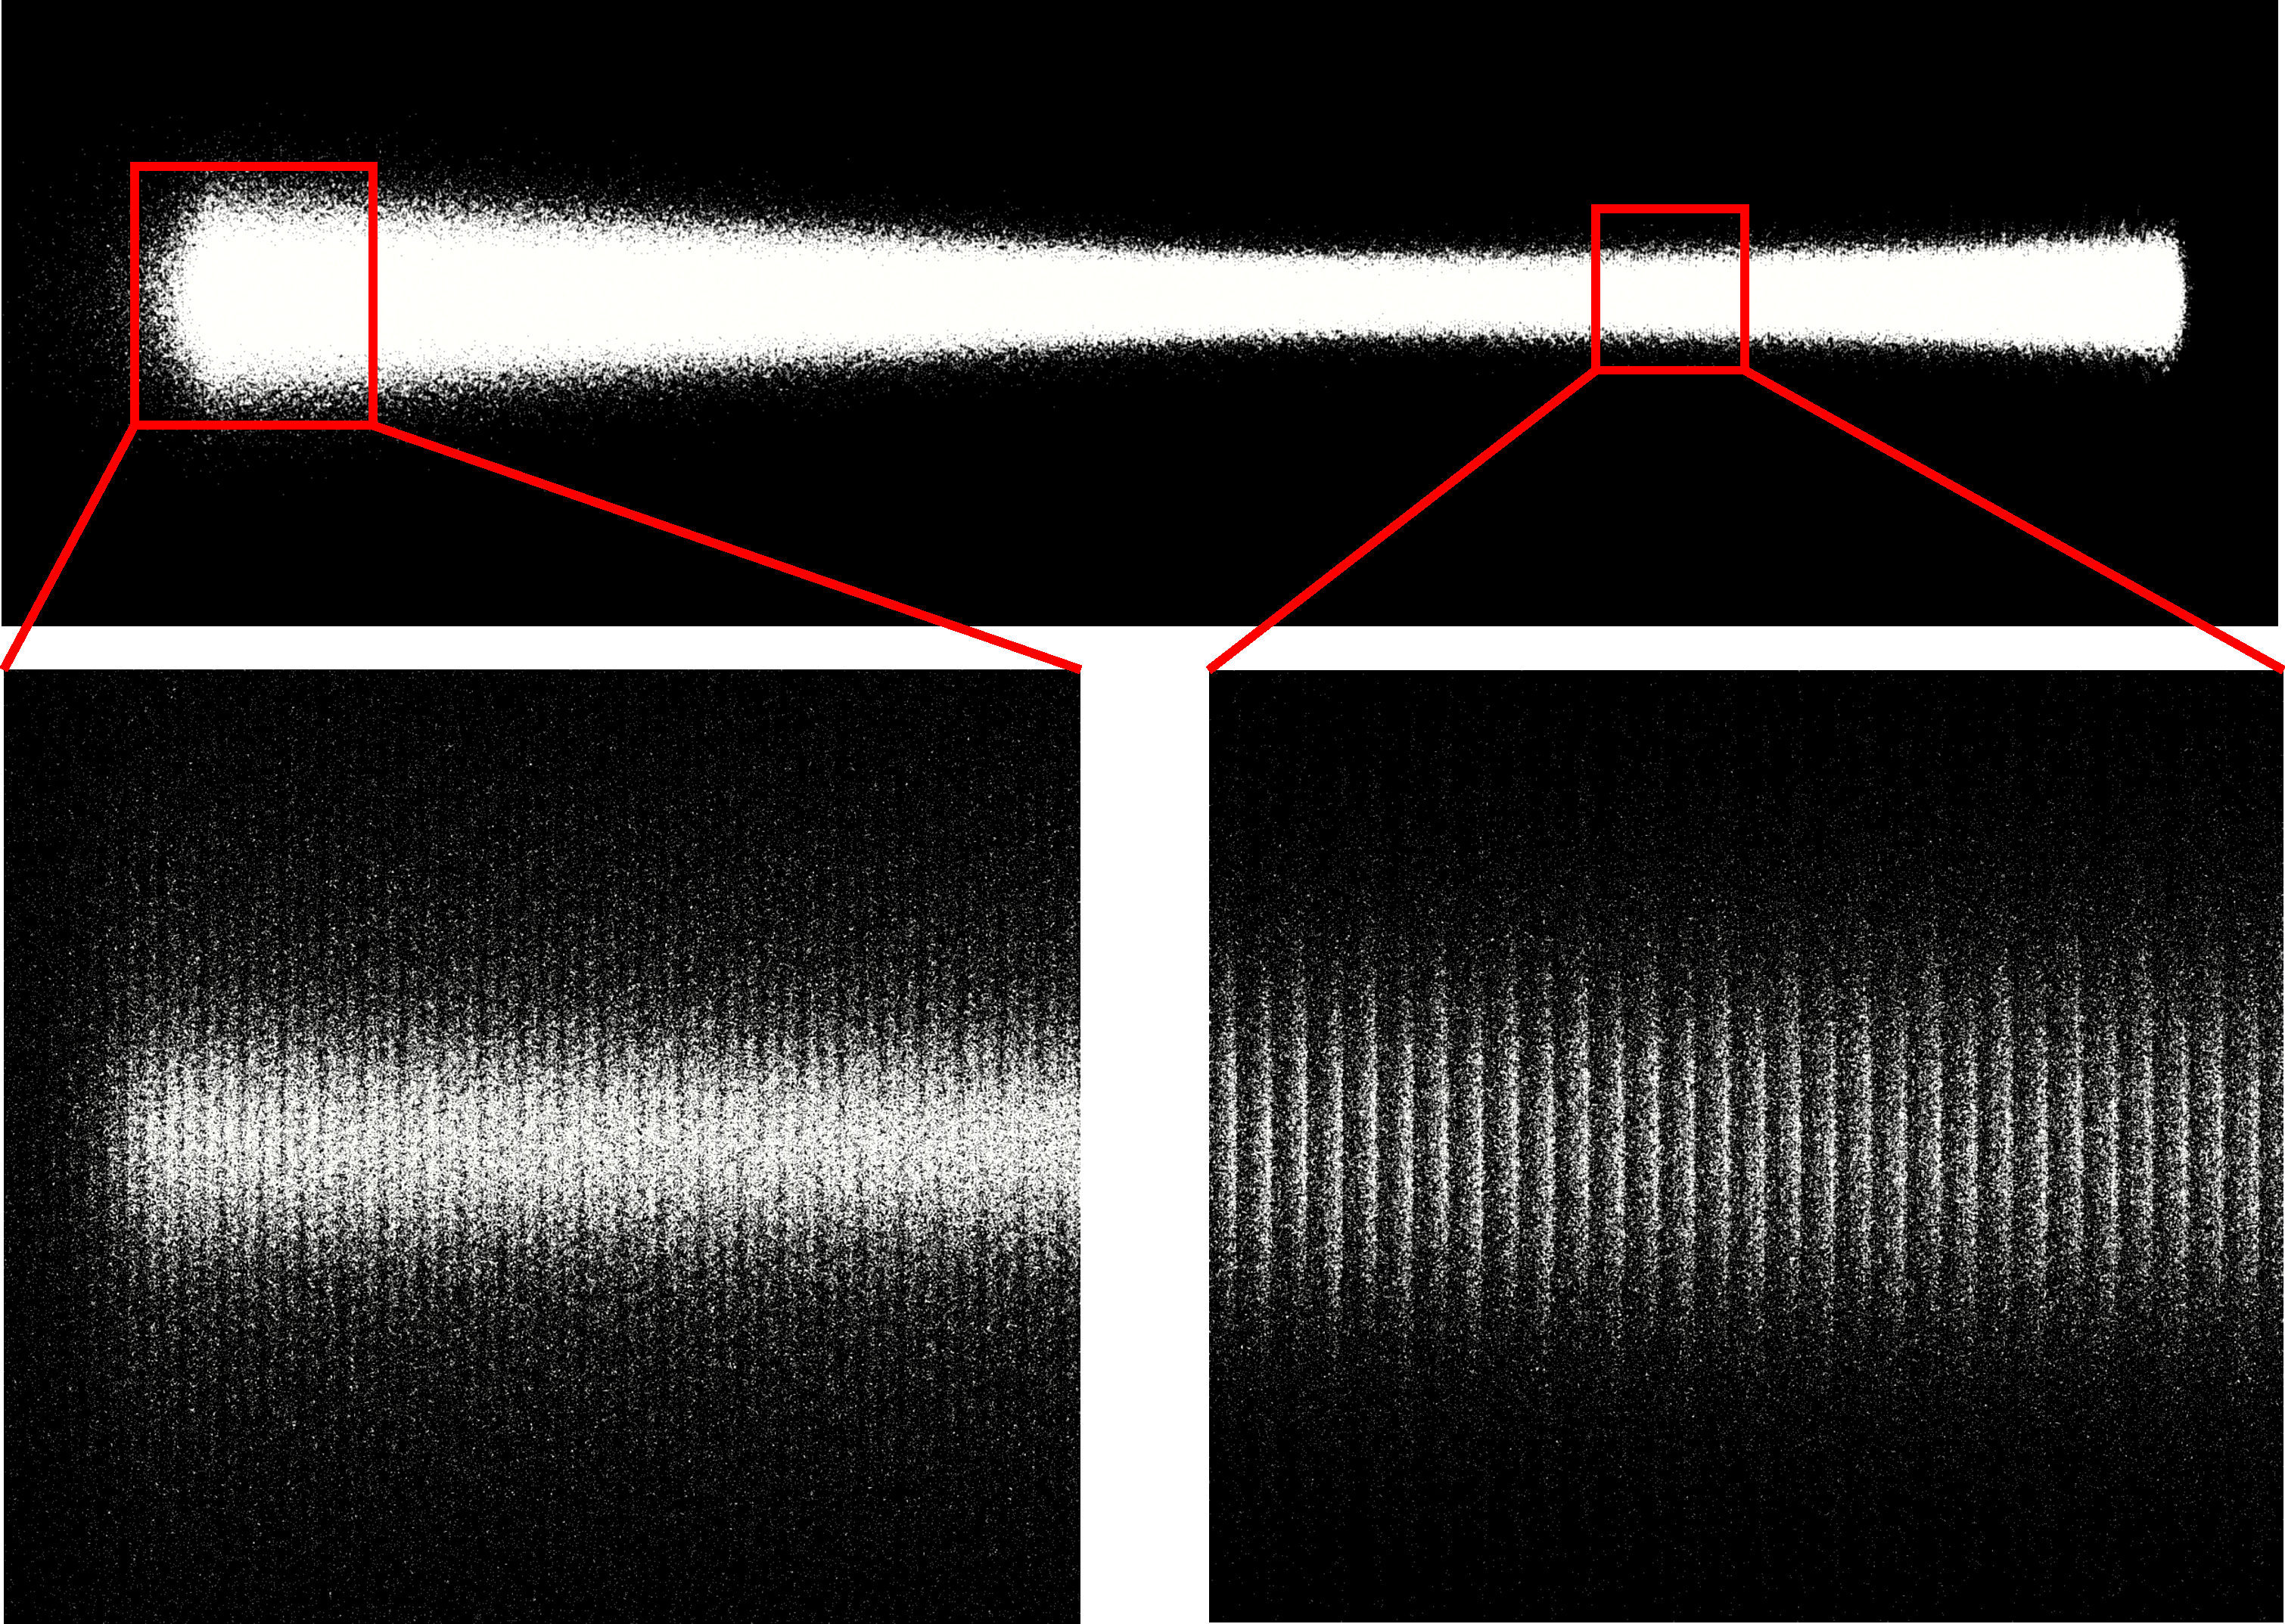
\includegraphics[height=2.5in]{./MITHRA_EXAMPLES/Fig6/Fig6b.pdf} \\
(a) & (b)
\end{array}$
\caption{(a) The total radiated power measured at 80\,$\mu$m distance from the bunch center in terms of the traveled undulator length and (b) the bunch profile at 12\,m from the undulator begin.}
\label{power-example2}
\end{figure}

\section{Example 3: Optical Undulator}

\subsection{Problem Definition}

As explained in the introduction of this manual, one of the milestones considered for the development of MITHRA is full-wave simulation of inverse Compton scattering (ICS) or the so-called optical undulator.
%
The possibility of lasing or the so-called micro-bunching in an electron beam due to an interaction with a counter-propagating laser beam has been under debate for several years.
%
A full-wave analysis of such an interaction definitely gives valuable physical insight to this process.
%
Note that the classical treatment of this interaction within MITHRA does not allow for any consideration of quantum mechanical effects.
%
It is known that the radiation of photons results in a backward force on electrons which leads to a change in their momenta.
%
In the spontaneous radiation regime, the ratio $\rho_1 = \hbar\omega/\gamma mc^2$, representing the amount of quantum recoil due to each photon emission, quantifies this effect.
%
In the FEL gain regime, $\rho_2 = (\hbar\omega/2 \rho_{FEL} \gamma mc^2)^2$, with $\rho_{FEL}$ being the FEL parameter, estimates the level of quantum recoil influence on the gain process \cite{bonifacio2006quantum,bonifacio2005quantum}.
%
The use of classical formulation for optical undulators is only valid if $\rho_1 \ll 1$ and $\rho_2 \ll 1$.

Before embarking on the analysis and interpretation of results for a typical ICS experiment, a benchmark to validate the analysis of optical undulators using FDTD/PIC is presented.
%
It is known that electron trajectories in a static undulator with undulator parameter $K$ and periodicity $\lambda_u$ are similar to the trajectories in an electromagnetic undulator setup with normalized vector potential $a_0=K$ and wavelength $\lambda_l=2\lambda_u$ \cite{esarey1993nonlinear}.
%
We take the first SASE FEL example in table \ref{example1} into account and analyze the same configuration but with an equivalent optical undulator.
%
For this purpose, the undulator definition of example 1 is entered according to the following:
%
\begin{snugshade}
\begin{Verbatim}[fontsize=\small, tabsize = 4]
UNDULATOR
{
  undulator-type                   = optical
  beam-type                        = plane-wave
  position                         = ( 0.0, 0.0, 0.0 )
  direction                        = ( 0.0, 0.0,-1.0 )
  polarization                     = ( 0.0, 1.0, 0.0 )
  strength-parameter               = 1.417
  signal-type                      = flat-top
  wavelength                       = 6.0e4
  variance                         = 1800.0e4
  offset                           = 9000150
  CEP                              = 0.0
}
\end{Verbatim}
\end{snugshade}
%
Fig.\,\ref{ICS-benchmark} illustrates a comparison between the radiated infrared light for the static and optical undulator cases.
%
The very close agreement between the two results validates the implementation of optical undulators in MITHRA.
%
\begin{figure}
\centering
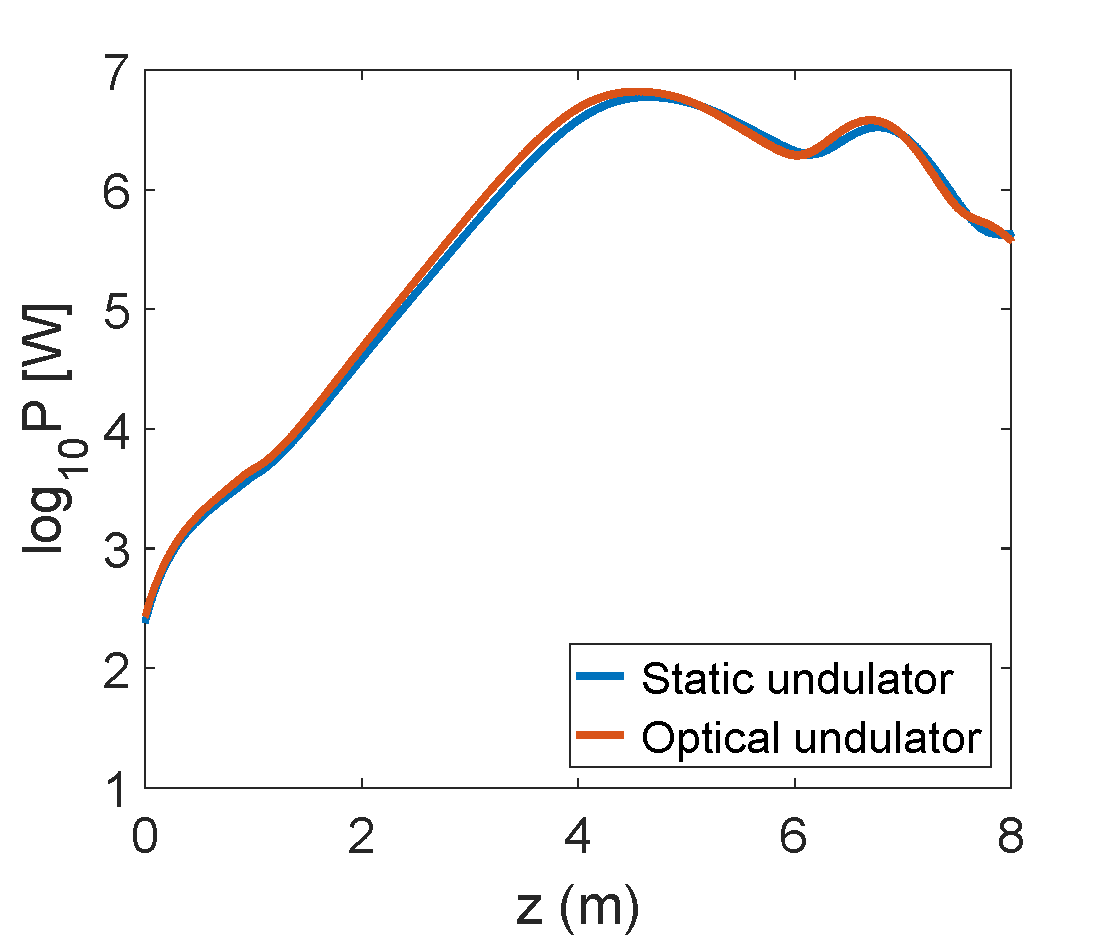
\includegraphics[height=2.5in]{./MITHRA_EXAMPLES/Fig7/Fig7.pdf}
\caption{The total radiated power calculated at 110\,$\mu$m distance from the bunch center in terms of the traveled undulator length compared for two cases of an optical and static undulator.}
\label{ICS-benchmark}
\end{figure}

The parameters of FEL interaction in an optical undulator, considered as the third example, are tabulated in table \ref{example3}.
%
Since we observe drastic deviation from the predictions of one-dimensional FEL theory in our simulations, we have not listed the FEL parameters calculated using the 1D theory.
%
We believe the discrepancies are originated from the small number of electrons in each 3D wave bucket, i.e. only 2 electrons.
%
This strongly intensifies the 3D effects, dramatically reduces the transverse coherence of the radiation, and indeed makes analysis using 1D FEL theory completely invalid.
%
We comment that for the listed parameters $\rho_1=2\times10^{-4}$ and $\rho_2=0.003$, which are much smaller than errors caused by space-time discretization.
%
\begin{table}
\label{example3}
\caption{Parameters of the FEL configuration with optical undulator considered as the third example.}
\centering
\begin{tabular}{|c||c|}
\hline
FEL parameter & Value \\ \hline \hline
Current profile & Uniform \\ \hline
Bunch size & $(60\times60\times144)$\,nm \\ \hline
Bunch charge & 0.45\,fC \\ \hline
Bunch energy & 15\,MeV \\	\hline
Bunch current & 0.93\,A \\ \hline
Longitudinal momentum spread & 0.1\% \\ \hline
Normalized emittance & 1.75 nm-rad \\	\hline
Laser wavelength & 1\,$\mu$m \\ \hline
Laser strength parameter & 1.0 \\ \hline
Pulse duration & 4\,ps \\ \hline
Laser pulse type & flat-top \\ \hline
Radiation wavelength & 0.41\,nm \\ \hline
Electron density & $5.4\times10^{18} 1/\text{cm}^3$ \\ \hline
Initial bunching factor & $0.0$ \\ \hline
\end{tabular}
\end{table}

To simulate the considered FEL configuration, the following job file is written and given to the software to analyze the interaction.
%
\begin{snugshade}
\begin{Verbatim}[fontsize=\small, tabsize = 4]
MESH
{
  length-scale                     = NANOMETER
  time-scale                       = ATTOSECOND
  mesh-lengths                     = ( 2000.0, 2000.0, 165.0 )
  mesh-resolution                  = (    5.0,    5.0,   0.05)
  mesh-center                      = (    0.0,    0.0,   0.0 )
  total-time                       = 2000000
  bunch-time-step                  = 20.0
  bunch-time-start                 = 0.0
  mesh-truncation-order            = 2
  space-charge                     = true
}

BUNCH
{
  bunch-initialization
  {
    type                           = ellipsoid
    distribution                   = uniform
    charge                         = 2800
    number-of-particles            = 2800
    gamma                          = 30.0
    direction                      = (  0.0,   0.0,   1.0)
    position                       = (  0.0,   0.0,   0.0)
    sigma-position                 = ( 60.0,  60.0,  72.0)
    sigma-momentum                 = ( 0.03,  0.03,  0.03)
    transverse-truncation          = 240.0
    longitudinal-truncation        = 77.0
    bunching-factor                = 0.0
  }
}

FIELD
{
  field-sampling
  {
    sample                         = true
    type                           = at-point
    field                          = Ex
    field                          = Ey
    field                          = Ez
    directory                      = ./
    base-name                      = field-sampling/field
    rhythm                         = 3.2
    position                       = (0.0, 0.0, 110.0)
  }
}

UNDULATOR
{
  undulator-type                   = optical
  beam-type                        = plane-wave
  position                         = ( 0.0, 0.0, 0.0 )
  direction                        = ( 0.0, 0.0,-1.0 )
  polarization                     = ( 0.0, 1.0, 0.0 )
  strength-parameter               = 0.5
  signal-type                      = flat-top
  wavelength                       = 1.0e3
  variance                         = 1200.0e3
  offset                           = 600082.0
  CEP                              = 0.0
}

FEL-OUTPUT
{
  radiation-power
  {
    sample                         = true
    type                           = at-point
    directory                      = ./
    base-name                      = power-sampling/power
    distance-from-bunch            = 82
    normalized-frequency           = 1.000
    normalized-frequency           = 2.000
    normalized-frequency           = 3.000
  }
}
\end{Verbatim}
\end{snugshade}

\subsection{Simulation Results}

Fig.\,\ref{power-example3}a illustrates the radiation field 82\,nm away from the bunch center.
%
In addition, Fig.\,\ref{power-example3}b shows the radiated power in terms of travelled undulator distance computed using MITHRA, illustrating the effect of space charge and energy spread.
%
It is observed that the gain obtained in this regime is very small compared with a usual static undulators.
%
The reason for this effect is the very large shot noise in the bunch because of the low number of particles in each micro-bunch.
%
Note that in this simulation, each electron is modeled as one single particle with quite loading assumption before entering the undulator.
%
The strong shot noise causes a strong initial radiation, which reaches the expected saturation power after a low gain.
%
As a matter of fact, the micro-bunching process increases the coherence of the output radiation rather than power amplification.
%
Another aspect in this regime of interaction is the generation of strong higher order harmonics, which are depicted up to the third harmonic in Fig.\,\ref{power-example3}c.
%
Note that the accuracy of the results decreases for higher harmonics due to the required resolution in the computational mesh.
%
To show that the micro-bunching effect takes place in this regime as well, the bunching factor of the electron beam is depicted in Fig.\,\ref{power-example3}d.
%
The bunching of the electrons due to the ICS interaction is clearly observed in the plot of bunching factor.
%
The investigation of bunching factor throughout the interaction shows that despite the low-gain, micro-bunching takes place. This micro-bunching process increases the longitudinal coherence of the output radiation. However, due to very strong initial radiation no coherent amplification is observed.
%
According to the depicted power and pulse shape, total number of emitted photons is approximately equal to $4.2\times10^3$.
%
\begin{figure}
\centering
$\begin{array}{cc}
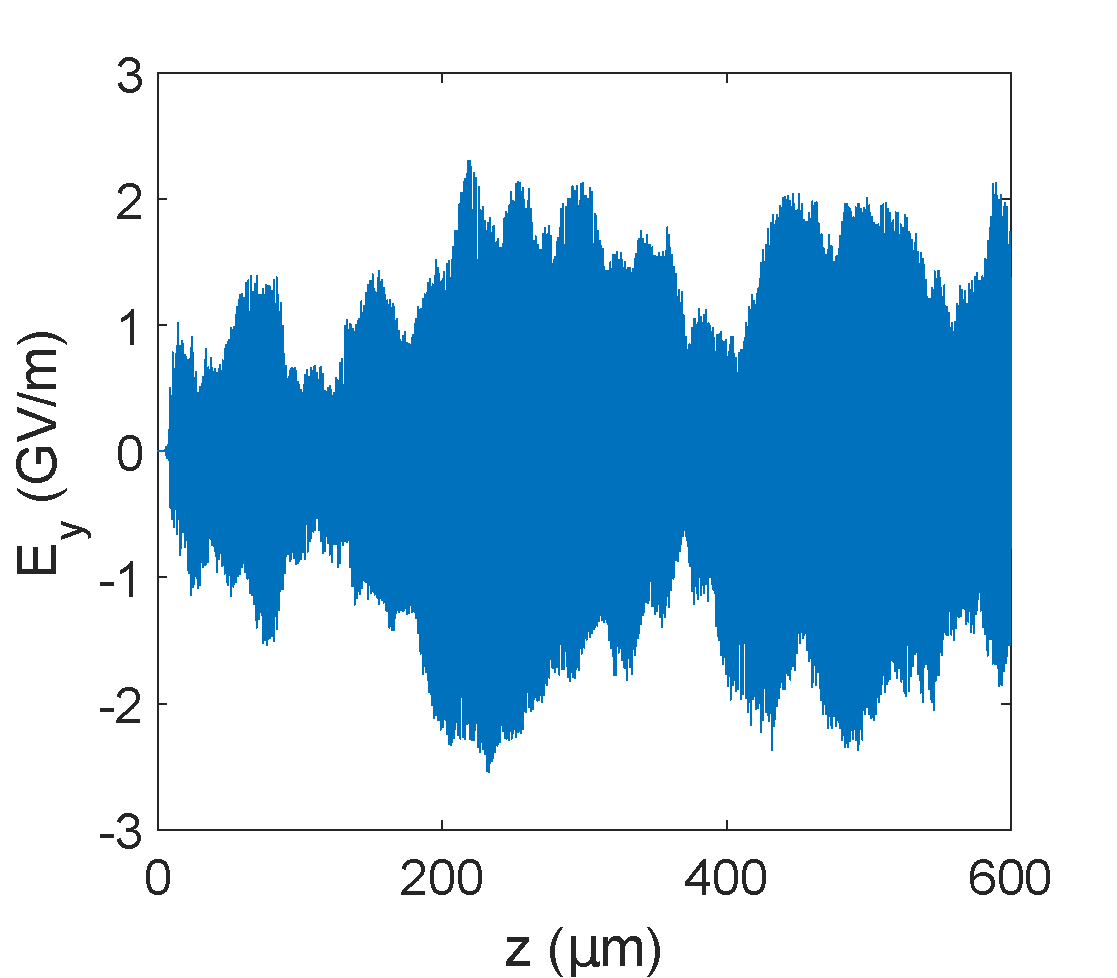
\includegraphics[height=2.5in]{./MITHRA_EXAMPLES/Fig8/Fig8a.pdf} & 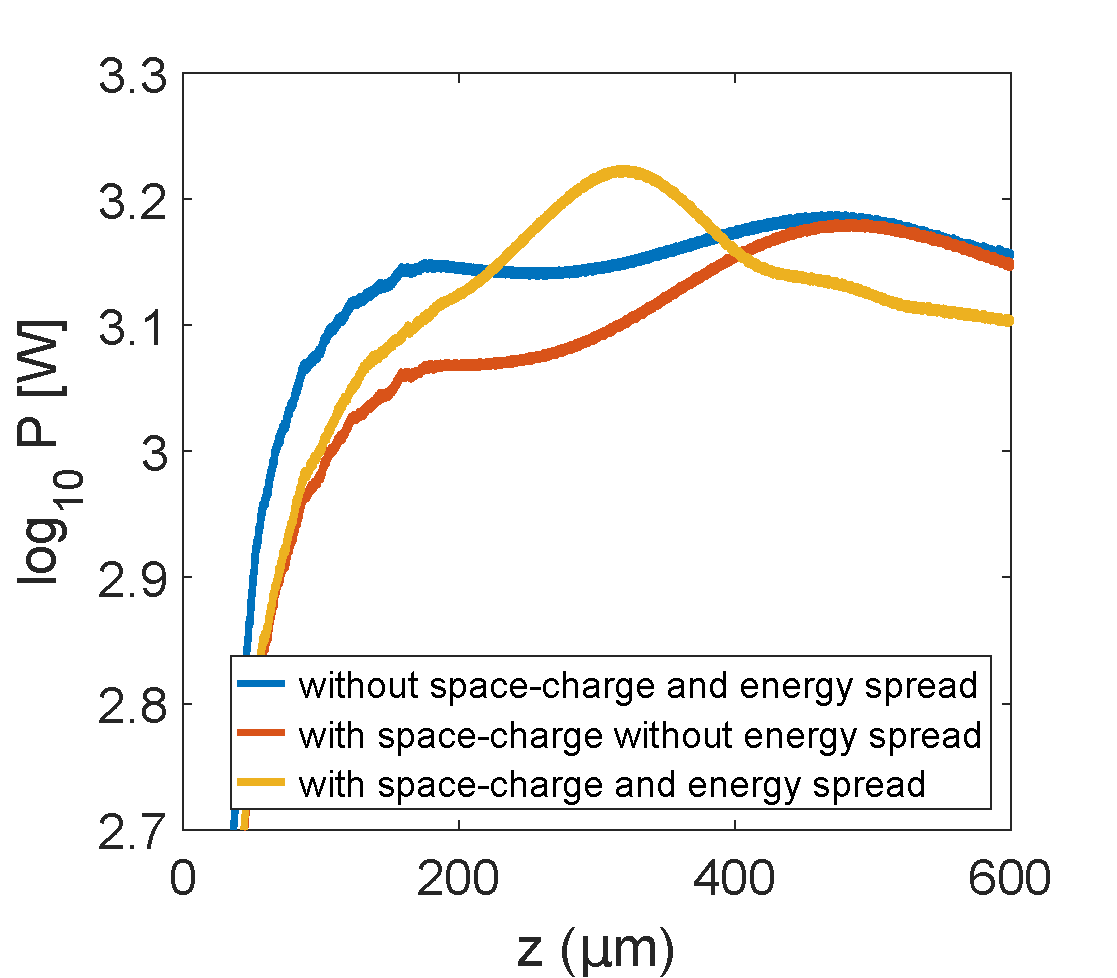
\includegraphics[height=2.5in]{./MITHRA_EXAMPLES/Fig8/Fig8b.pdf} \\
(a) & (b) \\
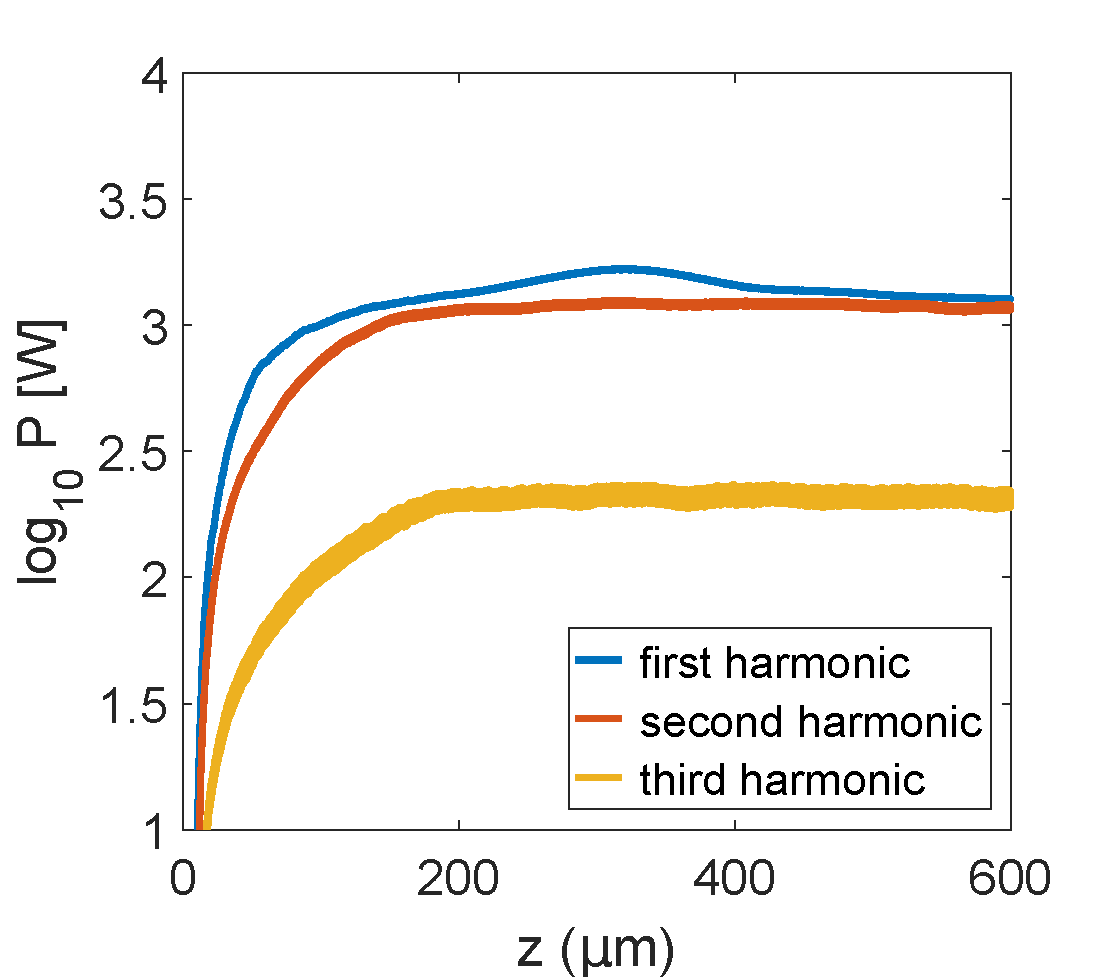
\includegraphics[height=2.5in]{./MITHRA_EXAMPLES/Fig8/Fig8c.pdf} & 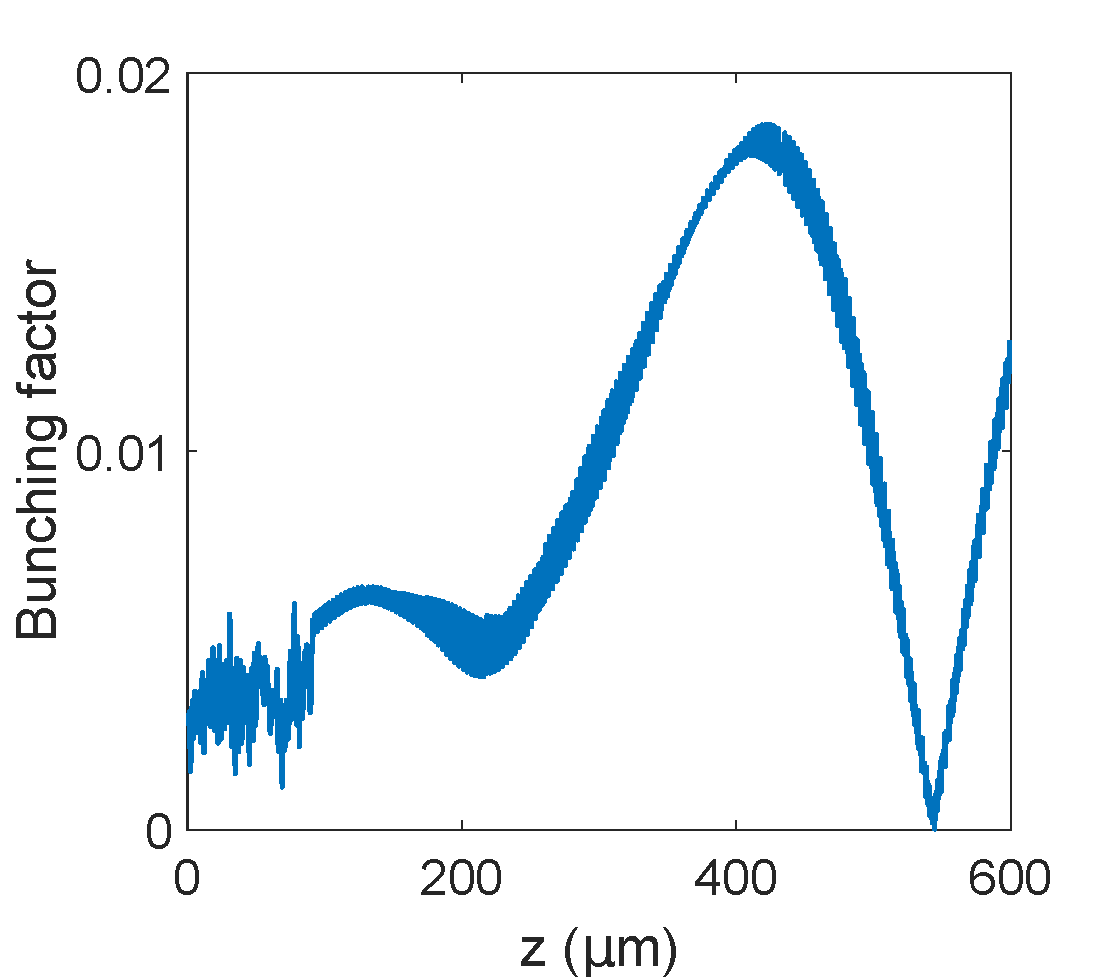
\includegraphics[height=2.5in]{./MITHRA_EXAMPLES/Fig8/Fig8d.pdf} \\
(c) & (d)
\end{array}$
\caption{(a) Electric field of the generated radiation in front of the bunch, (b) the total radiated power measured at 82\,nm distance from the bunch center in terms of the traveled distance, (c) the same radiation power for various harmonic orders, and (d) bunching factor of the considered bunch during the ICS interaction.}
\label{power-example3}
\end{figure}

To demonstrate the presented hypothesis related to the micro-bunching of bunches with low number of electrons per wavelength bucket, we perform an \emph{unreal} simulation, where each electron is presented by 1000 particles.
%
The thousand particles are distributed evenly throughout each wavelength bucket in order to drastically reduce the shot noise level.
%
In this case, each particle represents a charge 1000 times smaller than the charge of one electron.
%
In addition, we assume an initial bunching factor equal to 0.001 for the input bunch to trigger the FEL gain.
%
In Fig.\,\ref{powerUnreal-example3}, the radiation of such a charge configuration is depicted.
%
The results clearly reveal the radiation start from much lower powers, possibility of achieving the FEL gain and saturating in the same power level as above, thereby confirming the above theory for radiation of low density electron bunches.
%
Consequently, the presented simulation by MITHRA agrees with the already developed FEL theory, according to which low number of electrons per coherence volume prevents achieving the radiation gain, even if the electron bunch is micro-bunched.
%
\begin{figure}
\centering
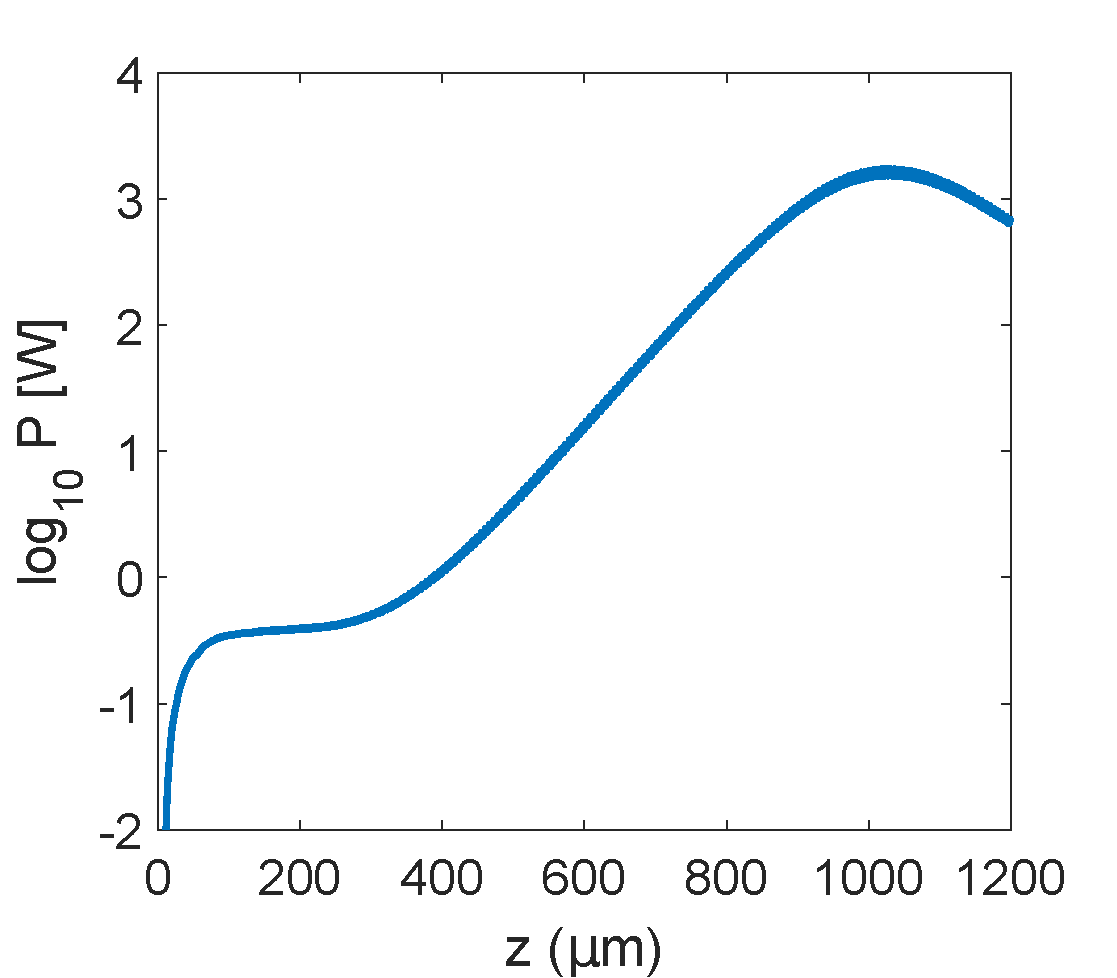
\includegraphics[height=2.5in]{./MITHRA_EXAMPLES/Fig9/Fig9.pdf}
\caption{The total radiated power measured at 82\,nm distance from the bunch center in terms of the traveled distance for an imaginary bunch where each electron is represented by a cloud of 1000 particles.}
\label{powerUnreal-example3}
\end{figure}

\section{Example 4: Free Propagation}

\subsection{Problem Definition}

The fourth example aims at verifying the implementation of space-charge forces in MITHRA.
%
For this purpose, we tackle the problem of free-space propagation for an electron bunch and study the bunch phase-space variations due to space-charge effect.
%
This problem can also be solved using well-established simulation tools in accelerator physics like ASTRA \cite{flottmann2011astra}.
%
We take the bunch of the first example, but with Gaussian distribution along the propagation path.
%
The computational domain needs to be slightly larger to account for the Gaussian distribution, and additionally no undulator parameter needs to be parsed to the solver.
%
The bunch sampling option in MITHRA is activated to save the statistical phase-space data during the propagation.
%
The job file to perform the above simulation in MITHRA will thus correspond to the following:
%
\begin{snugshade}
\begin{Verbatim}[fontsize=\small, tabsize = 4]
MESH
{
  length-scale                     = MICROMETER
  time-scale                       = PICOSECOND
  mesh-lengths                     = ( 3200,  3200.0,    350.0)
  mesh-resolution                  = ( 100.0,  100.0,      0.5)
  mesh-center                      = ( 0.0,      0.0,      0.0)
  total-time                       = 30000
  bunch-time-step                  = 1.6
  bunch-time-start                 = 0.0
  mesh-truncation-order            = 2
  space-charge                     = true
}

BUNCH
{
  bunch-initialization
  {
    type                           = ellipsoid
    distribution                   = gaussian
    charge                         = 1.846e8
    number-of-particles            = 262144
    gamma                          = 100.41
    direction                      = (    0.0,     0.0,       1.0)
    position                       = (    0.0,     0.0,       0.0)
    sigma-position                 = (  260.0,   260.0,     50.25)
    sigma-momentum                 = ( 1.0e-8,  1.0e-8, 100.41e-4)
    transverse-truncation          = 1040.0
    longitudinal-truncation        = 150.0
    bunching-factor                = 0.01
  }

  bunch-sampling
  {
    sample                         = true
    directory                      = ./
    base-name                      = bunch-sampling/bunchSC
    rhythm                         = 8
  }
}
\end{Verbatim}
\end{snugshade}

\subsection{Simulation Results}

In Fig.\,\ref{power-example4}, we show the results for the evolution of transverse bunch size as well as the divergence angle of the beam in root-mean-square (RMS).
%
As observed the bunch size expands with propagation along the undulator due to space-charge forces.
%
This is a confirmation for the considerable space-charge effect encountered in the first example.
%
The results obtained using both MITHRA and ASTRA are depicted and compared against each other.
%
The excellent agreement between the results evidences the reliability of the space-charge implementation in MITHRA.
%
\begin{figure}
\centering
$\begin{array}{cc}
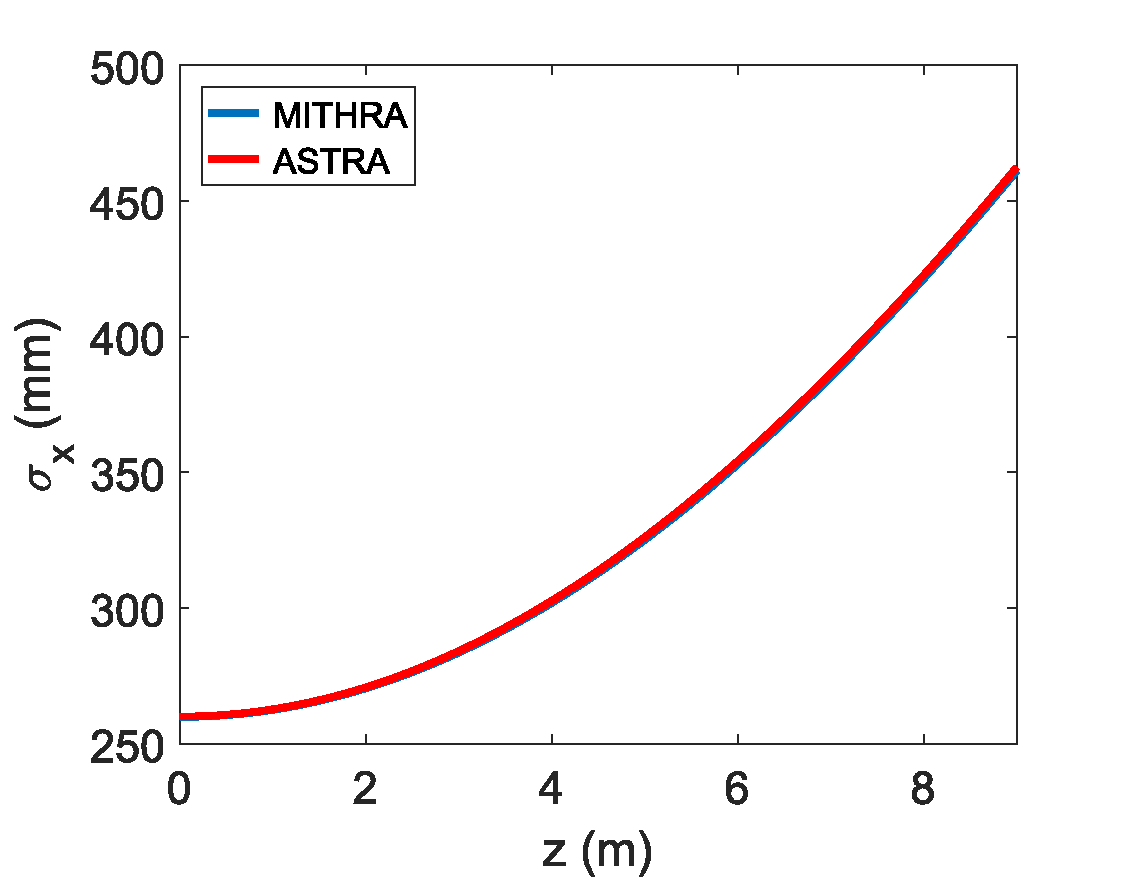
\includegraphics[height=2.5in]{./MITHRA_EXAMPLES/Fig10/Fig10a.pdf} & 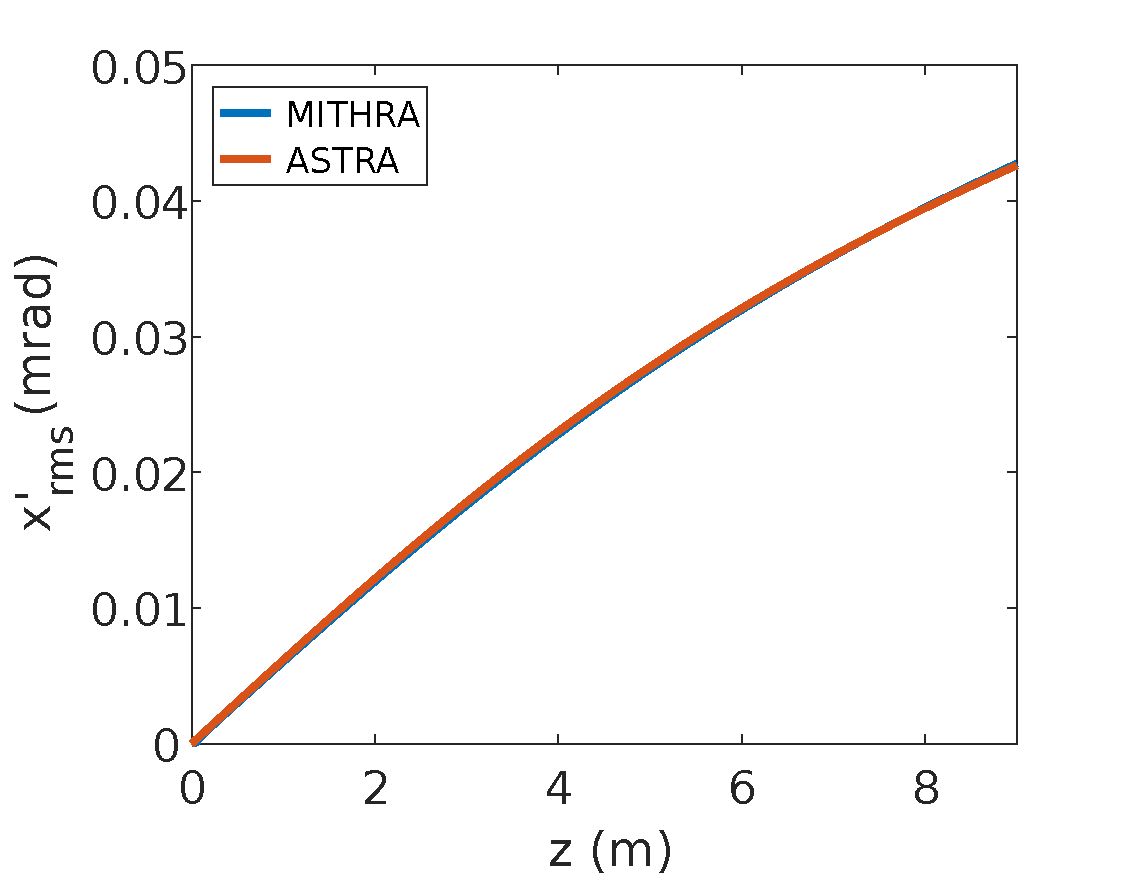
\includegraphics[height=2.5in]{./MITHRA_EXAMPLES/Fig10/Fig10b.pdf} \\
(a) & (b)
\end{array}$
\caption{(a) Transverse size and (b) rms divergence angle of the electron beam expanding due to space-charge forces after free propagation.}
\label{power-example4}
\end{figure}

\section{Example 5: Short Pulse Hard X-ray Source}

\subsection{Problem Definition}

\begin{table}
	\label{example5}
	\caption{Parameters of the hard X-ray FEL configuration considered as the fifth example.}
	\centering
	{\footnotesize
	\begin{tabular}{|c||c|}
		\hline
		FEL parameter & Value \\ \hline \hline
		Current profile & Uniform \\ \hline
		Bunch size & $(30.0\times30.0\times0.8)\,\mu$m \\ \hline
		Bunch charge & 20.0\,pC \\ \hline
		Bunch energy & 6.7\,GeV \\	\hline
		Bunch current & 7.5\,kA \\ \hline
		Longitudinal momentum spread & 0.1\% \\ \hline
		Normalized emittance & 0.2\,$\mu$m-rad \\	\hline
		Undulator period & 3.0\,cm \\ \hline
		Undulator parameter & 3.5 \\ \hline
		Undulator length & 40\,m \\ \hline
		Radiation wavelength & 0.62\,nm \\ \hline
		Gain length (1D) & 0.92\,m \\ \hline
		FEL parameter & 0.0015 \\ \hline
		Cooperation length & 19.3 nm \\ \hline
		Initial bunching factor & $0.0033$ \\ \hline
	\end{tabular}
	}	
\end{table}
%
In the fifth example, simulation of a problem with parameter sets corresponding to the short pulse regime of the hard X-ray FEL source in the LCLS facility is pursued.
%
The parameters considered in this example are tabulated in table \ref{example5}.
%
To simulate the described FEL, the following job file needs to be parsed in MITHRA.
%
\begin{snugshade}
\begin{Verbatim}[fontsize=\small, tabsize = 4]
MESH
{
  length-scale                     = MICROMETER
  time-scale                       = PICOSECOND
  mesh-lengths                     = ( 3200,  3200.0,    350.0)
  mesh-resolution                  = ( 100.0,  100.0,      0.5)
  mesh-center                      = ( 0.0,      0.0,      0.0)
  total-time                       = 30000
  bunch-time-step                  = 1.6
  bunch-time-start                 = 0.0
  mesh-truncation-order            = 2
  space-charge                     = true
}

BUNCH
{
  bunch-initialization
  {
    type                           = ellipsoid
    distribution                   = gaussian
    charge                         = 1.846e8
    number-of-particles            = 262144
    gamma                          = 100.41
    direction                      = (    0.0,     0.0,       1.0)
    position                       = (    0.0,     0.0,       0.0)
    sigma-position                 = (  260.0,   260.0,     50.25)
    sigma-momentum                 = ( 1.0e-8,  1.0e-8, 100.41e-4)
    transverse-truncation          = 1040.0
    longitudinal-truncation        = 150.0
    bunching-factor                = 0.01
  }

  bunch-sampling
  {
    sample                         = true
    directory                      = ./
    base-name                      = bunch-sampling/bunchSC
    rhythm                         = 8
  }
}
MESH
{
  length-scale                     = MICROMETER
  time-scale                       = PICOSECOND
  mesh-lengths                     = ( 400.0, 400.0,   1.5   )
  mesh-resolution                  = ( 4.0,     4.0,   3.0e-5 )
  mesh-center                      = ( 0.0,     0.0,   0.0    )
  total-time                       = 250000
  bunch-time-step                  = 1.6
  bunch-time-start                 = 0.0
  mesh-truncation-order            = 2
  space-charge                     = true
}

BUNCH
{
  bunch-initialization
  {
    type                           = ellipsoid
    distribution                   = uniform
    charge                         = 1.25e8
    number-of-particles            = 33554432
    gamma                          = 13089
    direction                      = ( 0.0,     0.0,  1.0)
    position                       = ( 0.0,     0.0,  0.0)
    sigma-position                 = ( 30.0,   30.0,  0.4)
    sigma-momentum                 = ( 0.007, 0.007, 13089e-3)
    transverse-truncation          = 180.0
    longitudinal-truncation        = 0.43
    bunching-factor                = 0.0033
  }
}

UNDULATOR
{
  undulator-type                   = static
  undulator-parameter              = 3.5
  period                           = 3.0e4
  length                           = 2500
  polarization-angle               = 0.0
}

FEL-OUTPUT
{
  radiation-power
  {
    sample                         = true
    type                           = at-point
    directory                      = ./
    base-name                      = power-sampling/power
    distance-from-bunch            = 0.45
    normalized-frequency           = 1.00
  }
}
\end{Verbatim}
\end{snugshade}

\subsection{Simulation Results}

Fig.\,\ref{power-example5} shows the computed radiated power in terms of traveled undulator distance with and without consideration of space-charge effects.
%
According to the 1D FEL theory, the FEL gain length for this example is around 0.92 m, which predicts saturation after around 18 m of undulator length.
%
However, due to 3D effects this saturation length is slightly longer than the predictions of 1D FEL theory.
%
Here, saturation length of about 22 m is observed for a space-charge free simulation.
%
In addition, the space-charge effect seems to be considerable after 10 m of undulator propagation, which contradicts with the typical assumptions that such effects are negligible for multi-GeV beams.
%
This large space-charge effect, not observed in the previous examples, is occurring due to the very short bunch length, which intensifies the Coulomb repulsion forces at the head and tail of the bunch.
%
A rough estimate of the Coulomb field leads to 1 V/m electric field, which in 10 meters of free propagation adds a displacement about 8 nm to the relativistic electrons.
%
This value being ten times larger than the radiation wavelength confirms the strong effect of space-charge forces.
%
In the beginning of the radiation, some artifacts are observed for the calculation with space-charge effect.
%
These artifacts are emerging because of the unrealistic modeling of fringing fields at the entrance of the undulator, which leads to nonzero magnetic field divergence.
%
To correct for such effects, numerical distribution of the fringing fields should be taken into account.
%
\begin{figure}
	\centering
	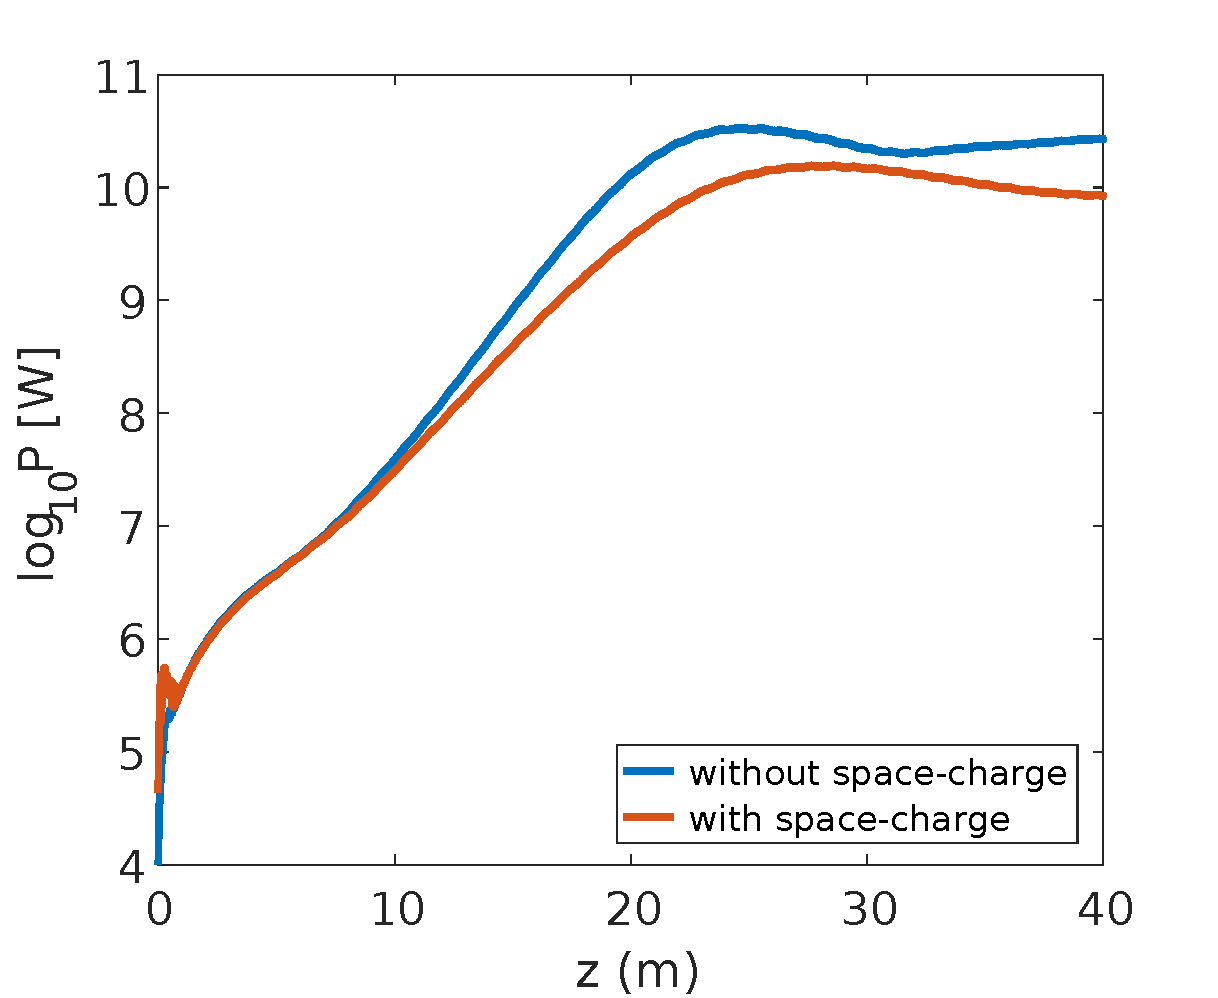
\includegraphics[height=2.5in]{./MITHRA_EXAMPLES/Fig11/Fig11.pdf} \\
    \caption{Total radiated power measured at 30\,nm distance from the bunch center in terms of the traveled undulator length for the hard X-ray FEL source as the third example.}
	\label{power-example5}
\end{figure}
